\documentclass[red,slidestop,notes,compress,mathserif]{beamer}

%\usepackage{beamerthemesplit}
\setbeamertemplate{navigation symbols}{}
\setbeamertemplate{note page}[plain]

\usetheme{Boadilla}
\usepackage{wasysym}
\usefonttheme{professionalfonts} % using non standard fonts for beamer
\usefonttheme{serif} % default family is serif
\usepackage{fontspec}

\usepackage{fontspec}
%\newfontfamily\greekfont[Mapping=tex-text]{DejaVu Serif}
%\setmainfont{Liberation Serif}


\title[CloudDP '15, Bordeaux]{V4VSockets: low-overhead intra-node communication in Xen.} 
\author[A. Nanos]{Anastassios Nanos, Stefanos Gerangelos, Ioanna Alifieraki, Nectarios Koziris}
\date{Apr. 21st, 2015}
\logo{
\includegraphics[scale=0.05]{figures/ntua_logo.pdf}
\includegraphics[scale=0.16]{figures/cslab_logo.pdf}}

\institute[CSLab, NTUA]{High-Performance Systems and Interconnects (HPSI),\\
Computing Systems Lab\\National Technical University of Athens\\
Github: \url{http://github.com/HPSI}\\
WWW: \url{http://cslab.ece.ntua.gr/research/}\\

\includegraphics[width=1.5cm]{figures/ntua_logo.pdf}

\includegraphics[width=3.5cm]{figures/cslab_logo.pdf}\\
%\includegraphics[angle=-90,width=4.0cm]{figs/hrakleitos.pdf}\\
}


\newcommand{\ta}{\insertframenumber}

\AtBeginSubsection[]
{
  \begin{frame}
  \frametitle{Overview}
  \tableofcontents[currentsection,currentsubsection]
  \end{frame}
}
\begin{document}


\frame{\titlepage}
\section*{Intro}

\begin{frame}
\frametitle{Intro}
\begin{block}{Cloud computing}
\begin{itemize}
\item application oriented
\item fast, ease-of-use
\end{itemize}
\end{block}
\begin{block}{Consolidation}
\begin{itemize}
\item $\frac{vCPU}{physical cores}$ $>>$ 1
\item multi/many--cores  
\end{itemize}
\end{block}
%\pause
\begin{block}{}
The number of co-located VMs is drastically increasing
\end{block}
%\pause
%\end{frame}

%\pause
\end{frame}

\begin{frame}
\frametitle{Introduction}
\begin{block}{Applications}
\begin{itemize}
\item stand-alone (flexibility)
\item distributed (elasticity)
\end{itemize}
When it comes to down to numbers, the need for intra-node communication in small data center increases.
\end{block}
\pause
\begin{block}{Contribution}

Design and Implement V4VSockets:
\begin{itemize}
\item efficient message exchange (one order of magnitude)
\item isolation
\item API compatible (Sockets)
\end{itemize}
\end{block}

\end{frame}


\section{Communication in Virtual Environments}

\subsection{Basic Concepts}

\begin{frame}
\frametitle{Xen - Architecture}
\begin{itemize}
\item hypervisor \& privileged VM (driver domain) to access hardware
\end{itemize}
\begin{figure}
\center
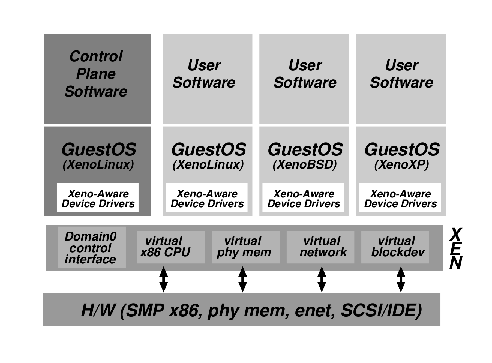
\includegraphics{figures/xen_arch.eps}
\end{figure}
\end{frame}

\section{I/O access in Virtualized Environments}

\subsection{Xen}
\begin{frame}
\frametitle{I/O Internals -- Xen}
\begin{block}{Xen basics}
                \begin{itemize}
                    \item hypervisor -- driver domain runs as a Linux guest
                    \item split driver model (frontend/backend)
                \end{itemize}
\end{block}
        \begin{block}{Xen -- Event channels}
                \begin{itemize}
                    \item notify Guest/Host about a pending transaction
                    \item easy to setup -- bind to a specific "port"
                \end{itemize}
        \end{block}
        \begin{block}{Xen -- Grant mechanism}
                \begin{itemize}
                    \item issue a page grant request
                    \item the other end maps the grant (accept)
                    \item this page is shared across the two domains
                \end{itemize}
        \end{block}

\end{frame}

\begin{frame}
\frametitle{Xen Ring buffers}
\begin{columns}
\column{\textwidth}
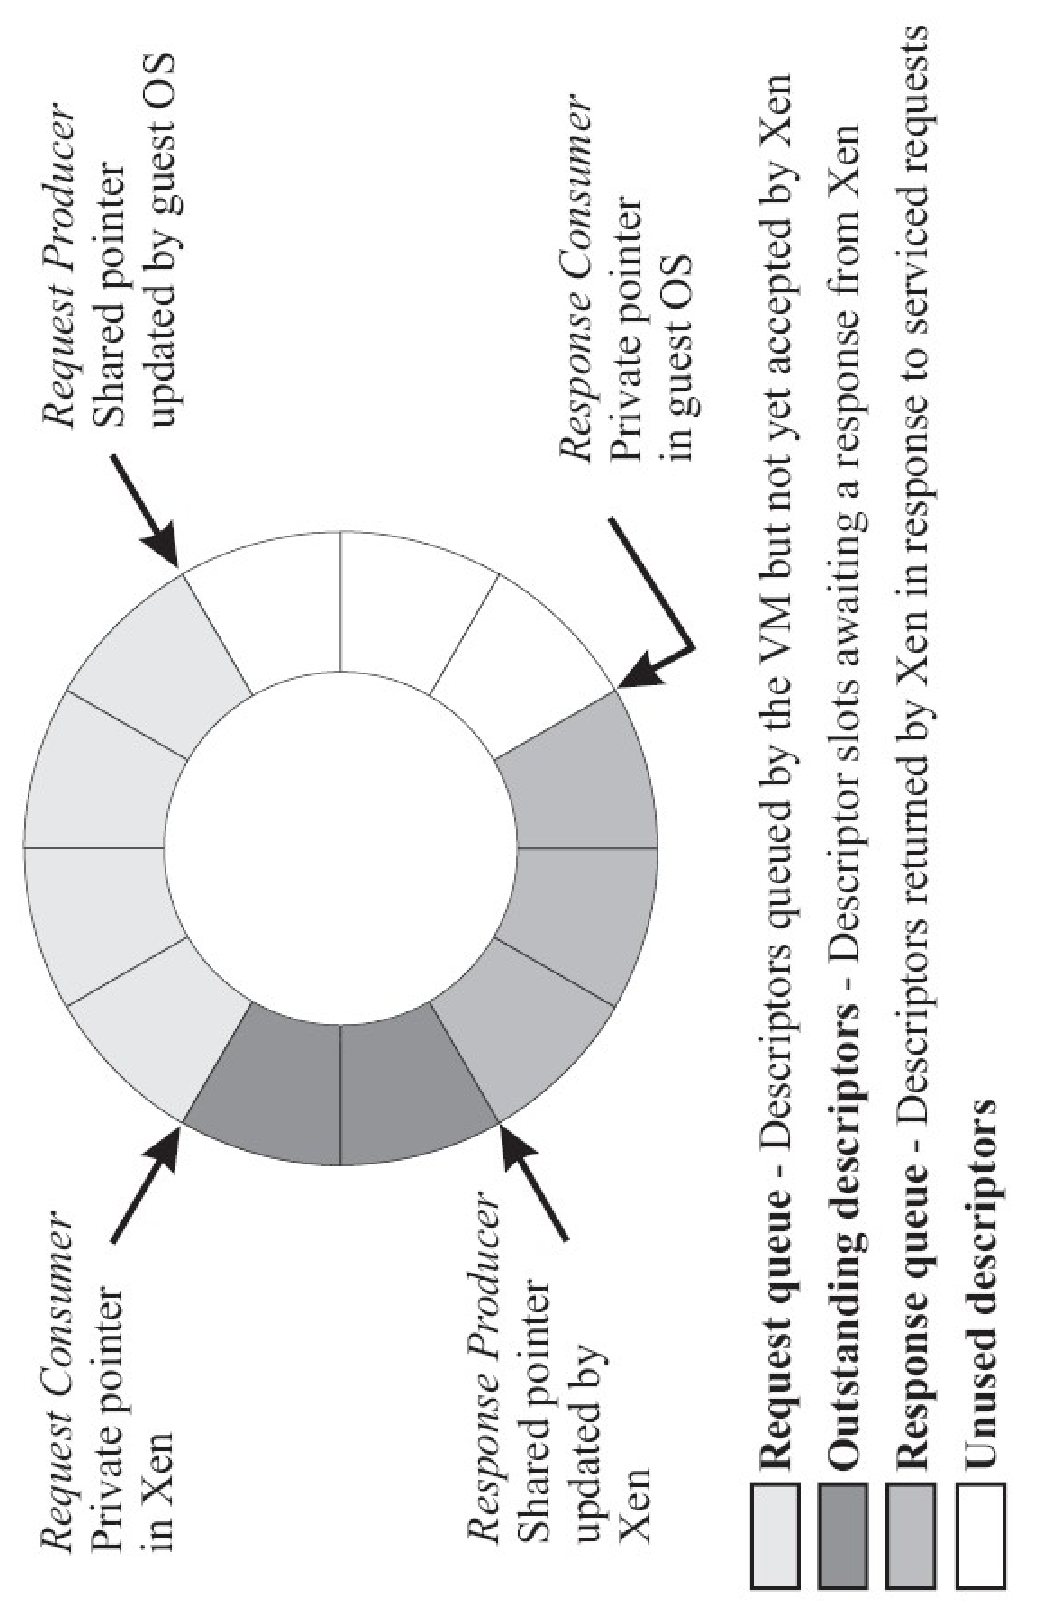
\includegraphics[width=.6\textwidth,angle=-90]{figures/test.eps}
\end{columns}
\end{frame}

%\begin{frame}
%\frametitle{Device Access - Split Driver Model}
%\begin{itemize}
%\item χρησιμοποιεί grant mechanism, event channels και ring buffers
%\item πραγματικός οδηγός
%\item κάτω μισό του διαχωρισμένου οδηγού (back-end)
%\item ring buffer
%\item πάνω μισό του διαχωρισμένου οδηγού (front-end)
%\end{itemize}
%%\begin{figure}
%%\includegraphics[scale=0.30]{figs/bare/io_paravirt.eps}
%%\end{figure}
%\end{frame}


\subsection{Intra-node communication in Xen}

\begin{frame}
\frametitle{Intra-node communication in Xen}
\begin{figure}
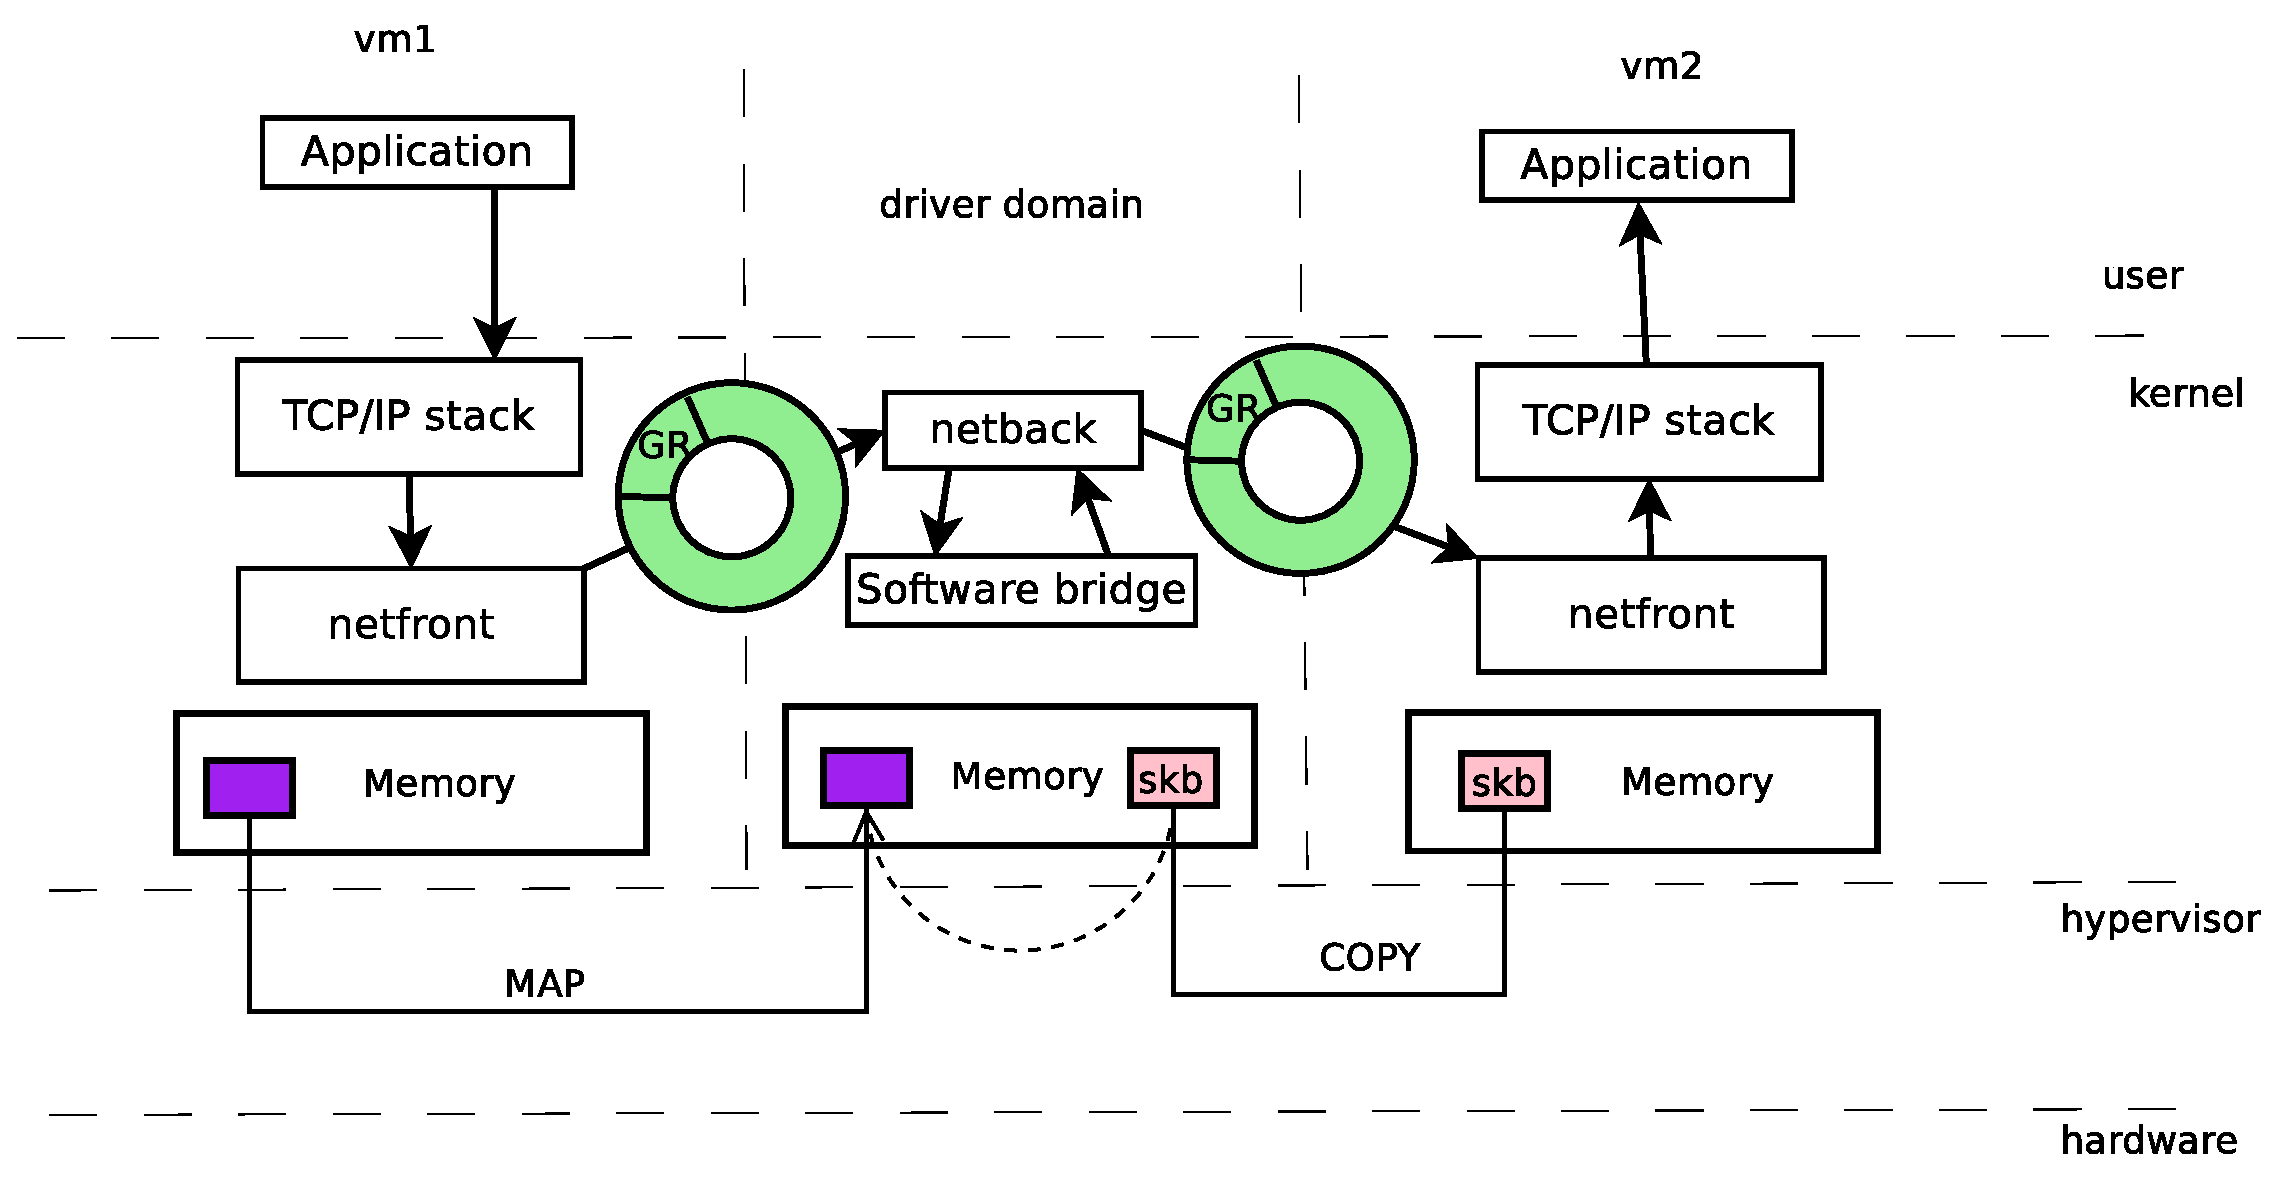
\includegraphics[width=\textwidth]{figures/netfront_netback.eps}
\end{figure}
\end{frame}


\section{V4VSockets}

\subsection{Architecture}

\begin{frame}
\frametitle{V4VSockets Architecture}
\begin{columns}
\column{.8\textwidth}
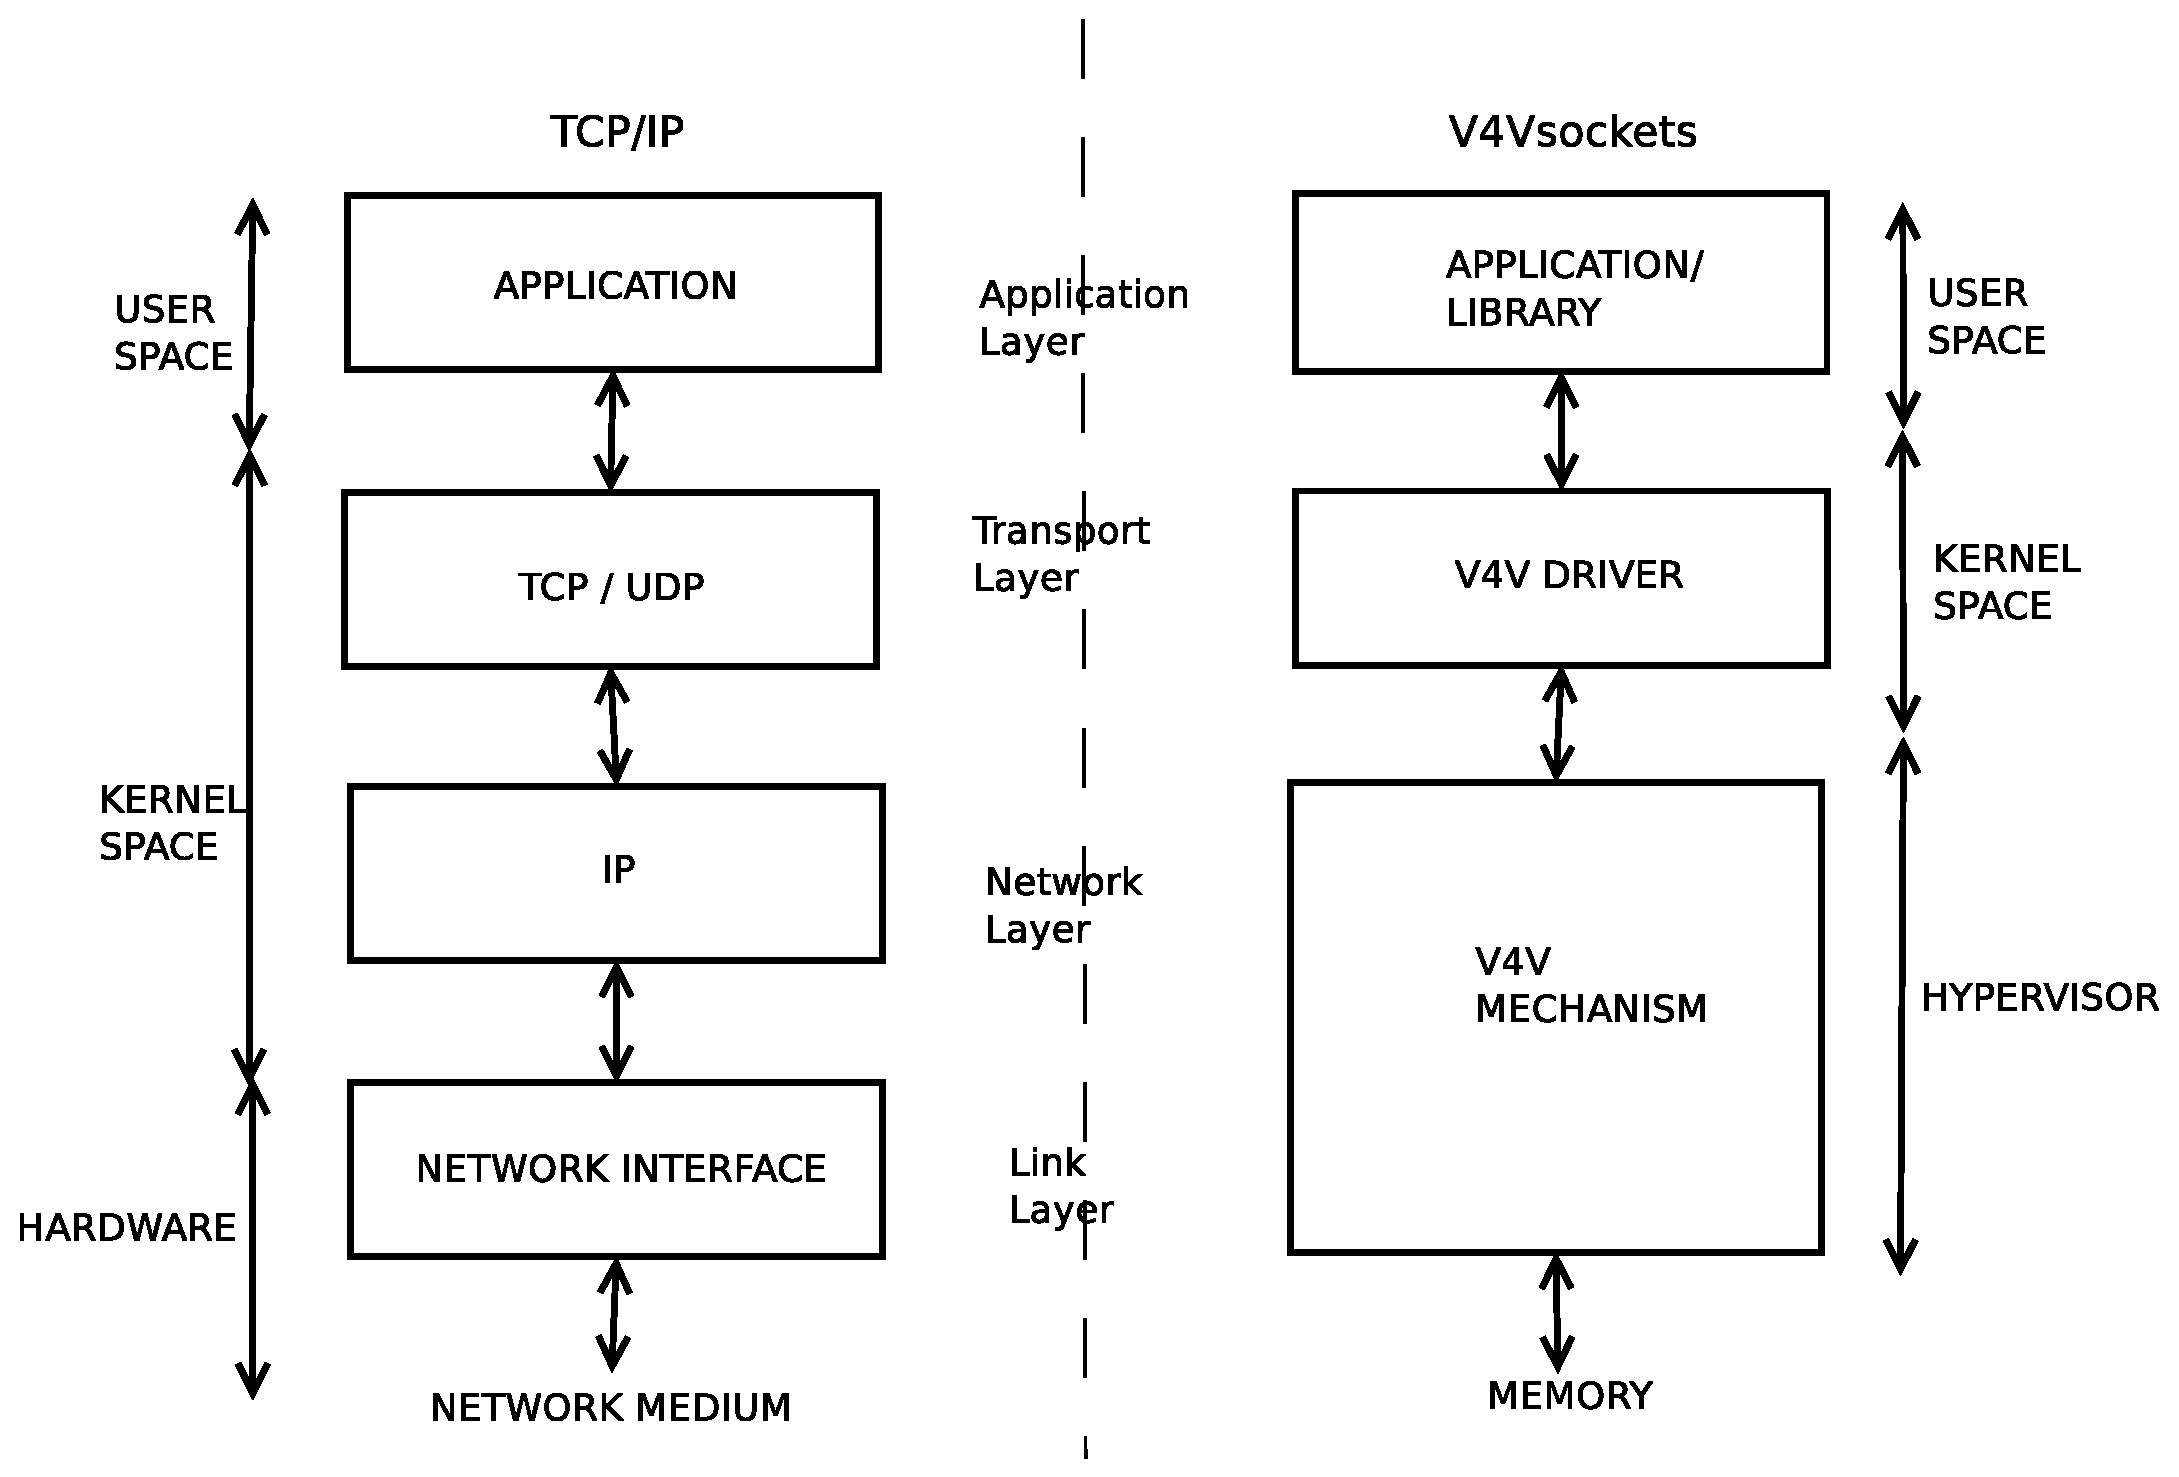
\includegraphics[width=\textwidth]{figures/tcp_ip_vs_v4vsockets.eps}
\end{columns}
\end{frame}

\begin{frame}
\frametitle{V4VSockets Architecture}
\begin{block}{Application/Library layer}
\begin{itemize}
\item forwards the relevant actions and arguments to the transport layer.
\end{itemize}
\end{block}
\end{frame}

\begin{frame}
\frametitle{V4VSockets Architecture}
\begin{block}{Transport layer -- V4V kernel driver}
\begin{itemize}
\item handles the virtual connection semantics between peer VMs that need to communicate,
\item is in charge of fragmenting and sending upper-layer packets by issuing hypercalls to the hypervisor (network layer), and
\item provides a notification mechanism to the VM's user-space for receiving packets, as well as error control.
\end{itemize}
\end{block}
\end{frame}

\begin{frame}
\frametitle{V4VSockets Architecture}
\begin{block}{Network/Link layer - Hypervisor}
\begin{itemize} 
\item encapsulation of upper-layer messages to packets that will be transmitted
to their destination, according to V4V semantics,
\item packet delivery.
\end{itemize}
\end{block}
\end{frame}

\begin{frame}
\frametitle{V4Vsockets vs Netfront/Netback}
\begin{figure}
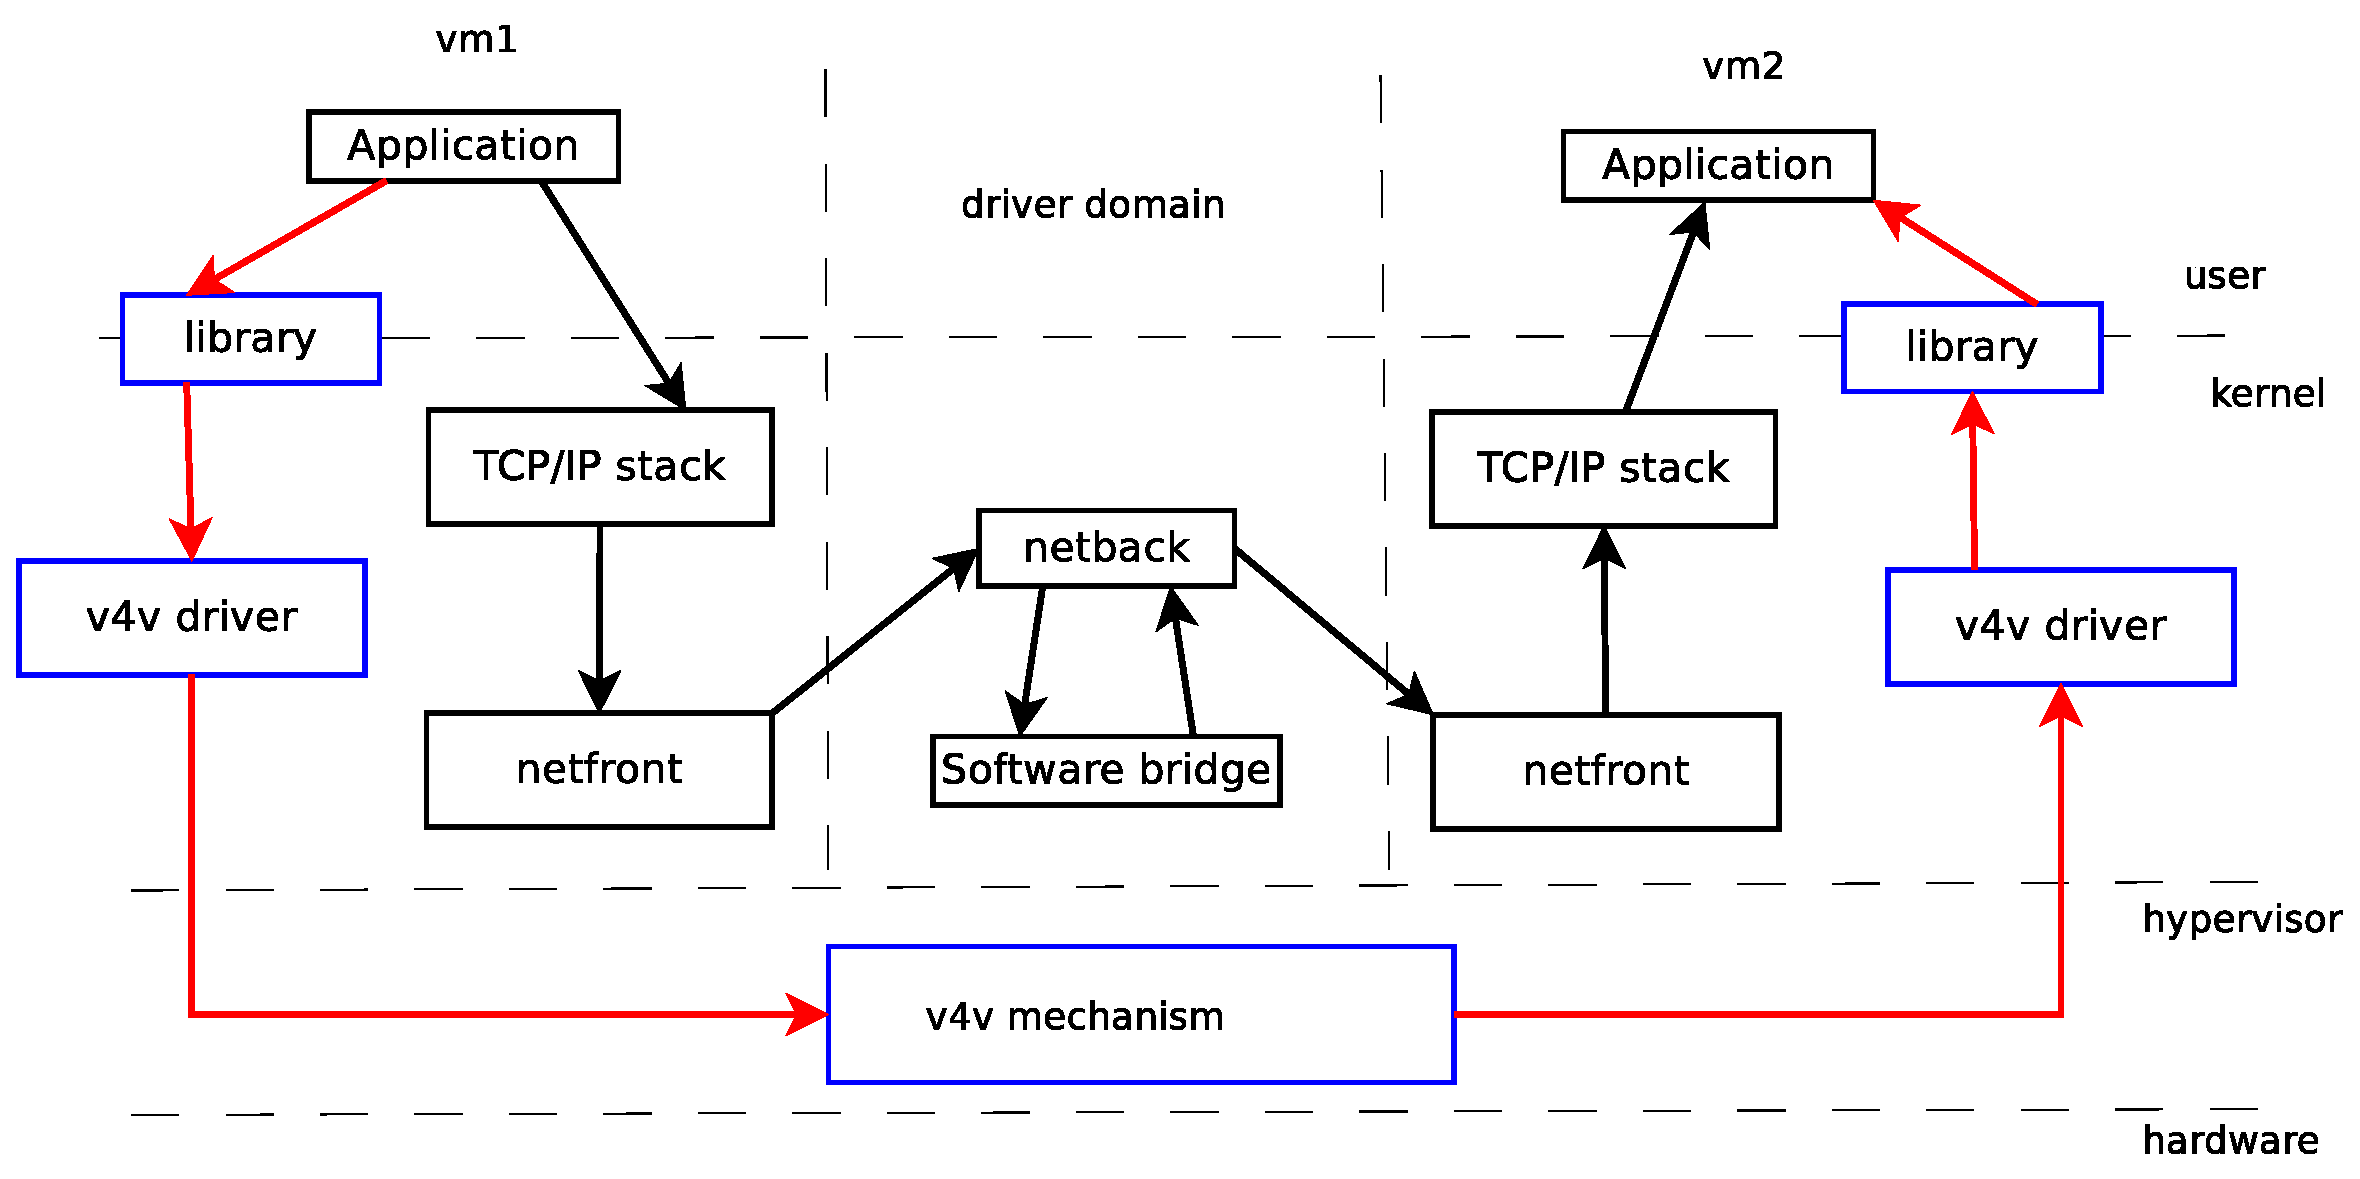
\includegraphics[width=\textwidth]{figures/paths.eps}
\end{figure}
\end{frame}

\begin{frame}
\frametitle{V4VSockets}       
\begin{block}{Communication mechanisms in V4VSockets}
\begin{itemize}
\item system calls 
\item hypercalls
\item event channels - VIRQS
\end{itemize}
\end{block}
\begin{block}{V4V Rings}
\begin{itemize}
\item circular buffers 
\item allocated in the VM address space by the VM kernel
\item data exchange medium
\end{itemize}
\end{block}
\end{frame}

\begin{frame}
\frametitle{V4VSockets -- Message Exchange}
\begin{figure}
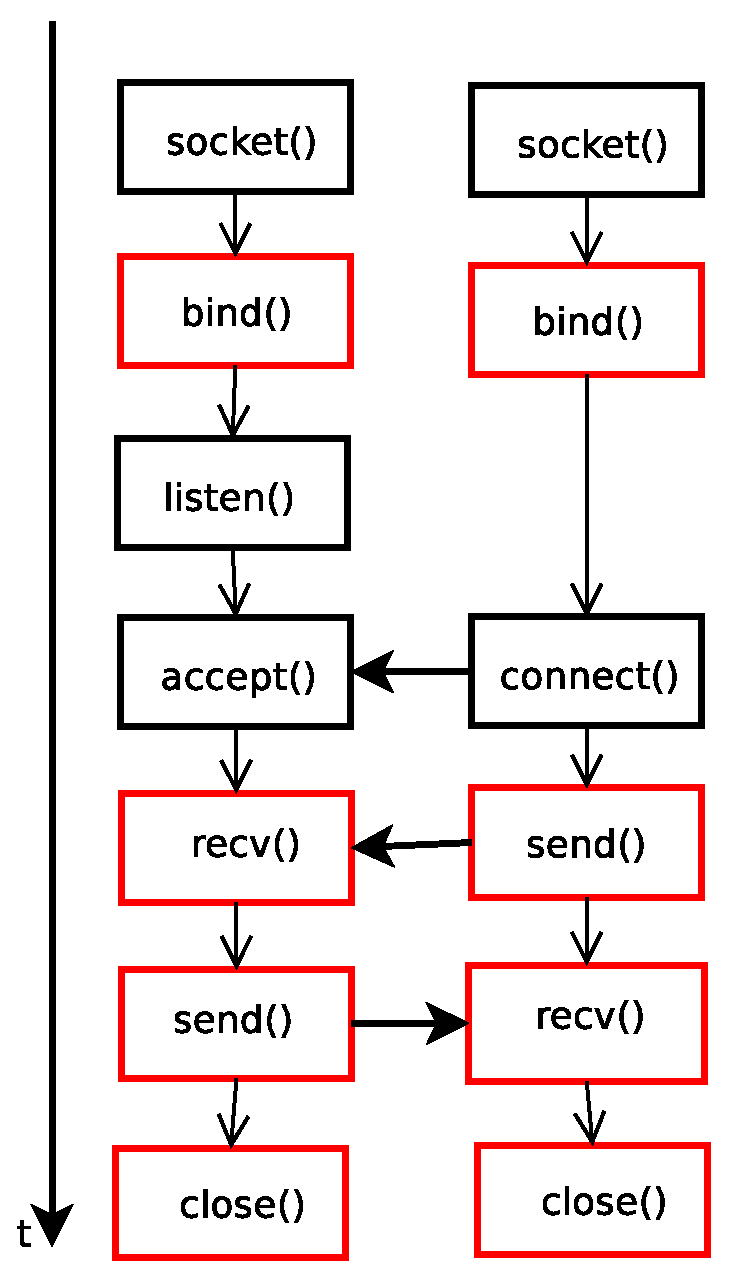
\includegraphics[scale=0.30]{figures/sockets.eps}
\end{figure}
\end{frame}

\begin{frame}
\frametitle{V4VSockets -- Message Exchange}
\begin{figure}
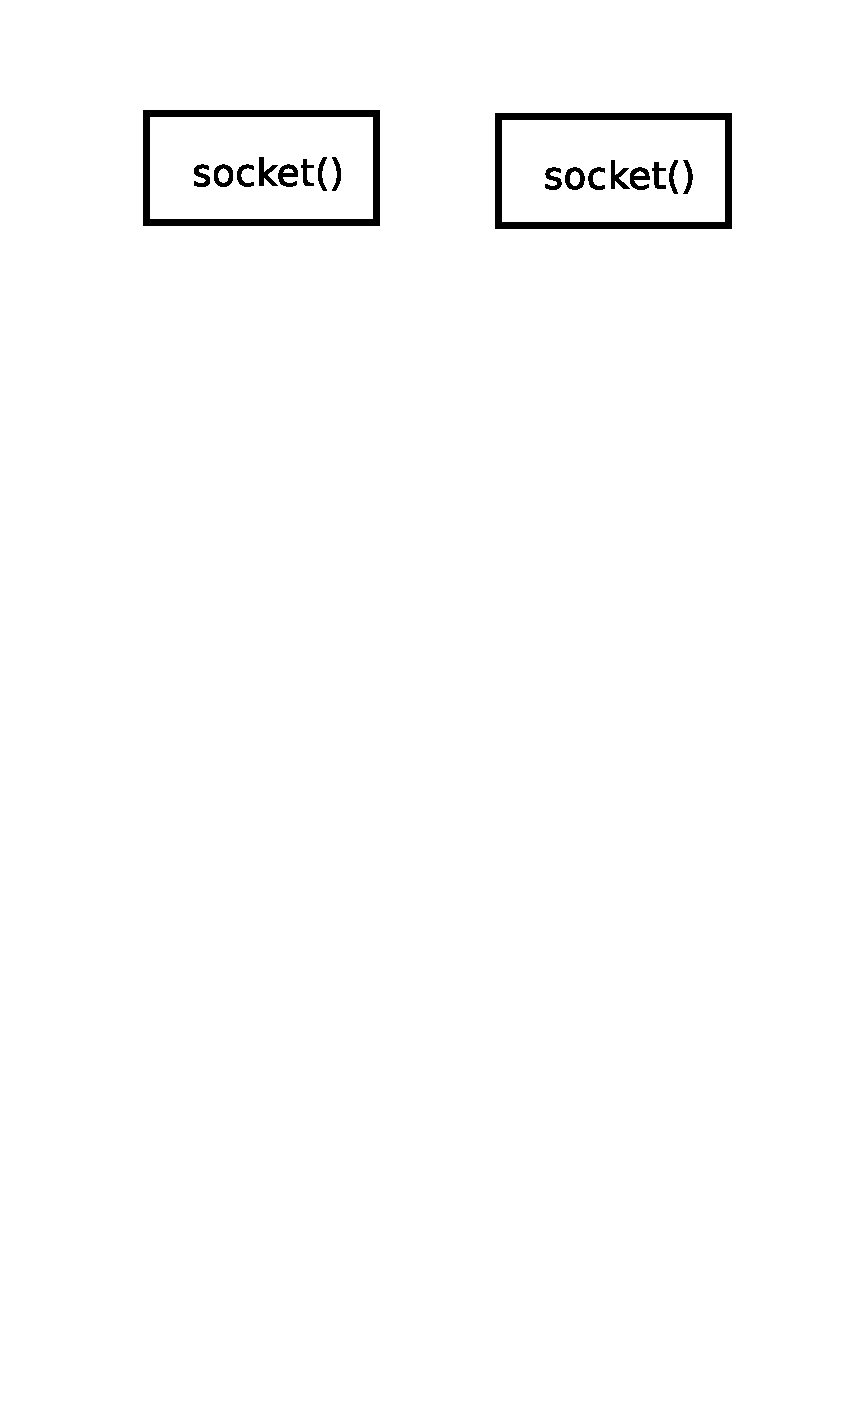
\includegraphics[scale=0.30]{figures/sockets6.eps}
\end{figure}
\end{frame}

\begin{frame}
\frametitle{V4VSockets -- Message Exchange}
\begin{figure}
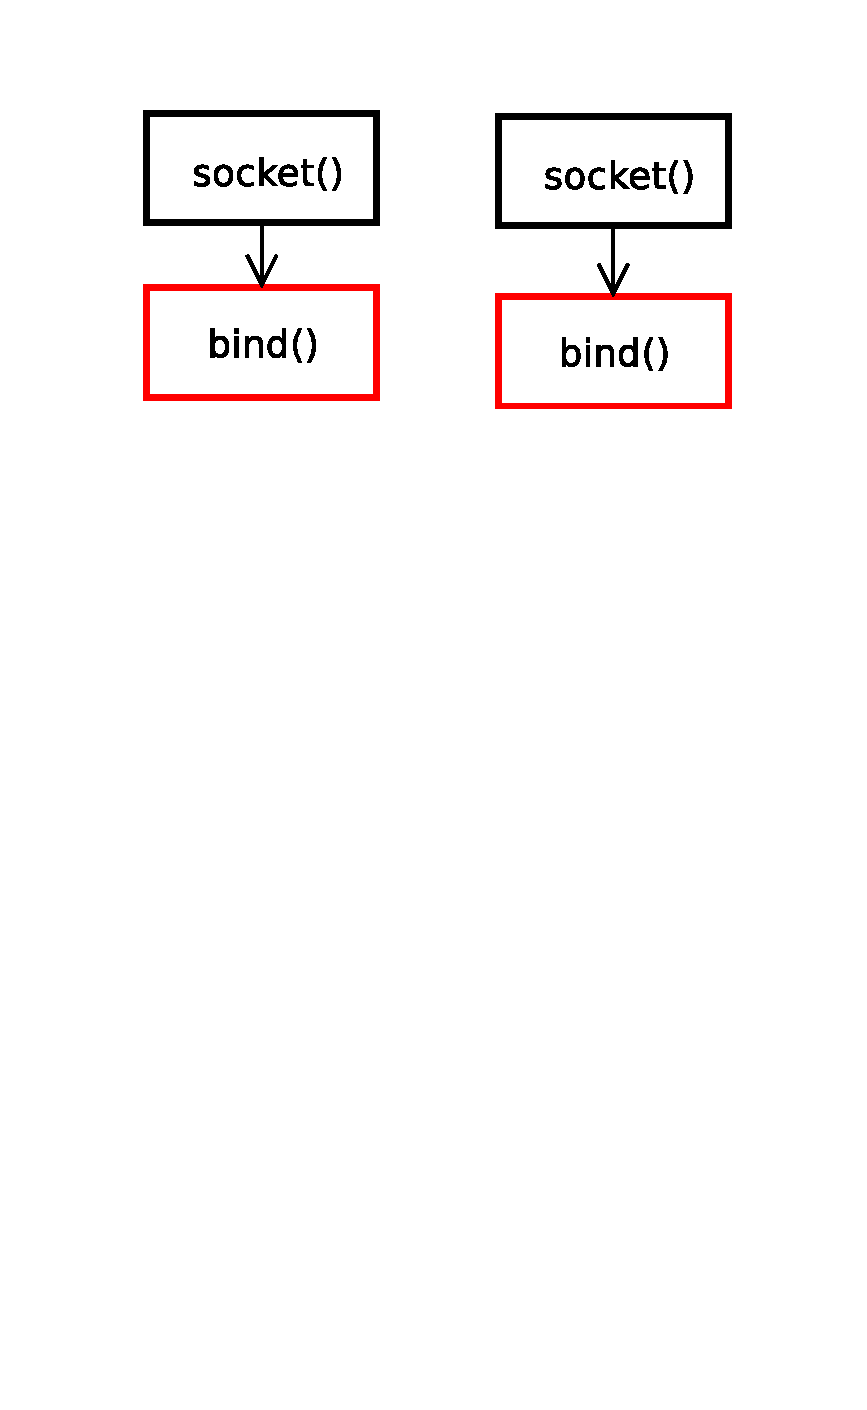
\includegraphics[scale=0.30]{figures/sockets5.eps}
\end{figure}
\end{frame}

\begin{frame}
\frametitle{V4VSockets -- Message Exchange}
\begin{figure}
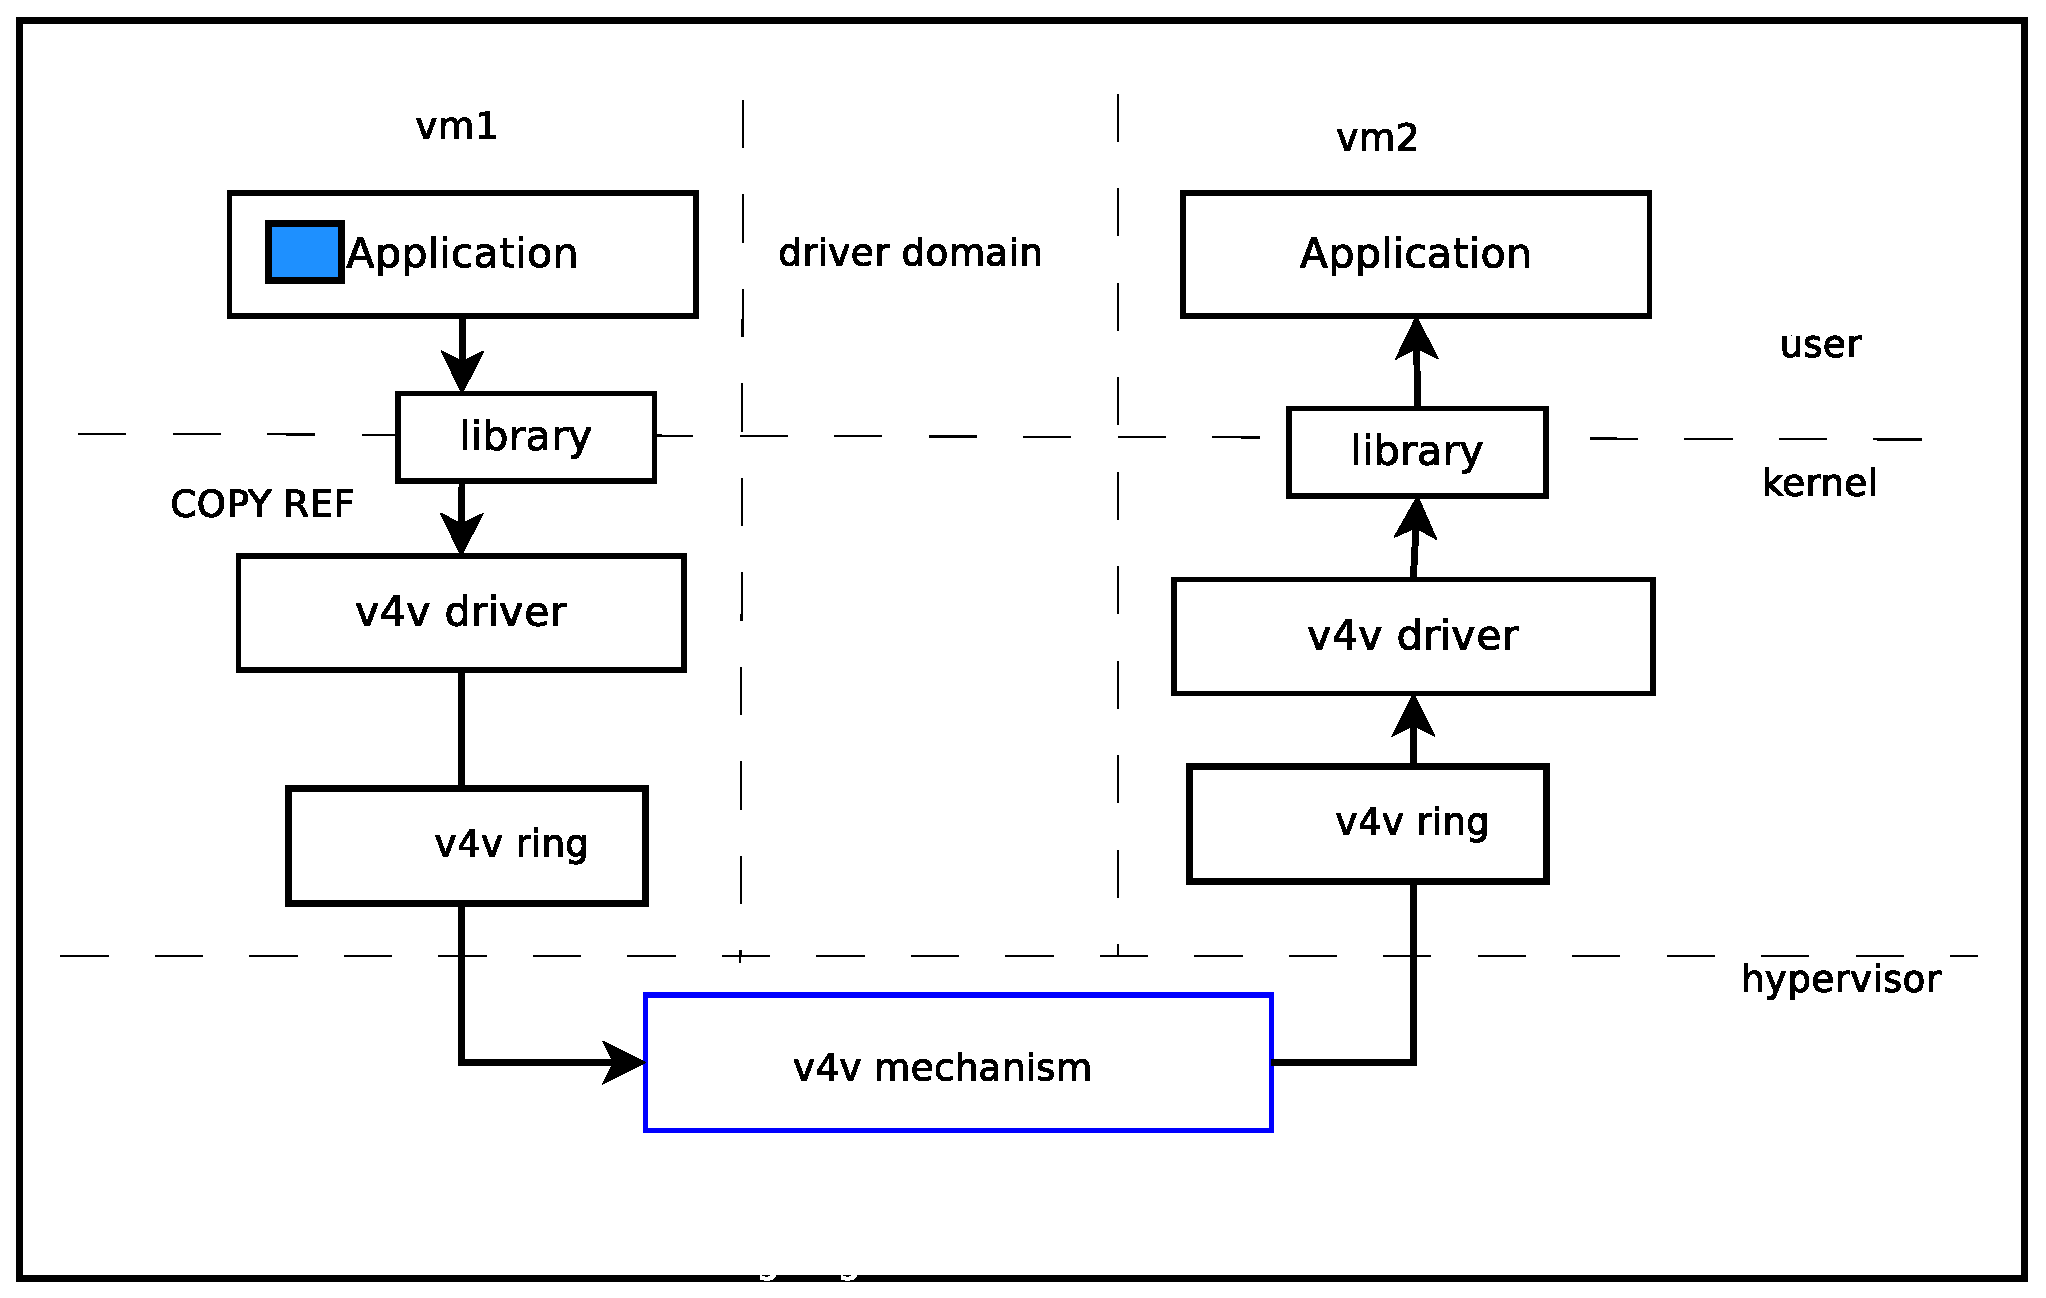
\includegraphics[scale=0.30]{figures/v4vsockets5.eps}
\end{figure}
\end{frame}

\begin{frame}
\frametitle{V4VSockets -- Message Exchange}
\begin{figure}
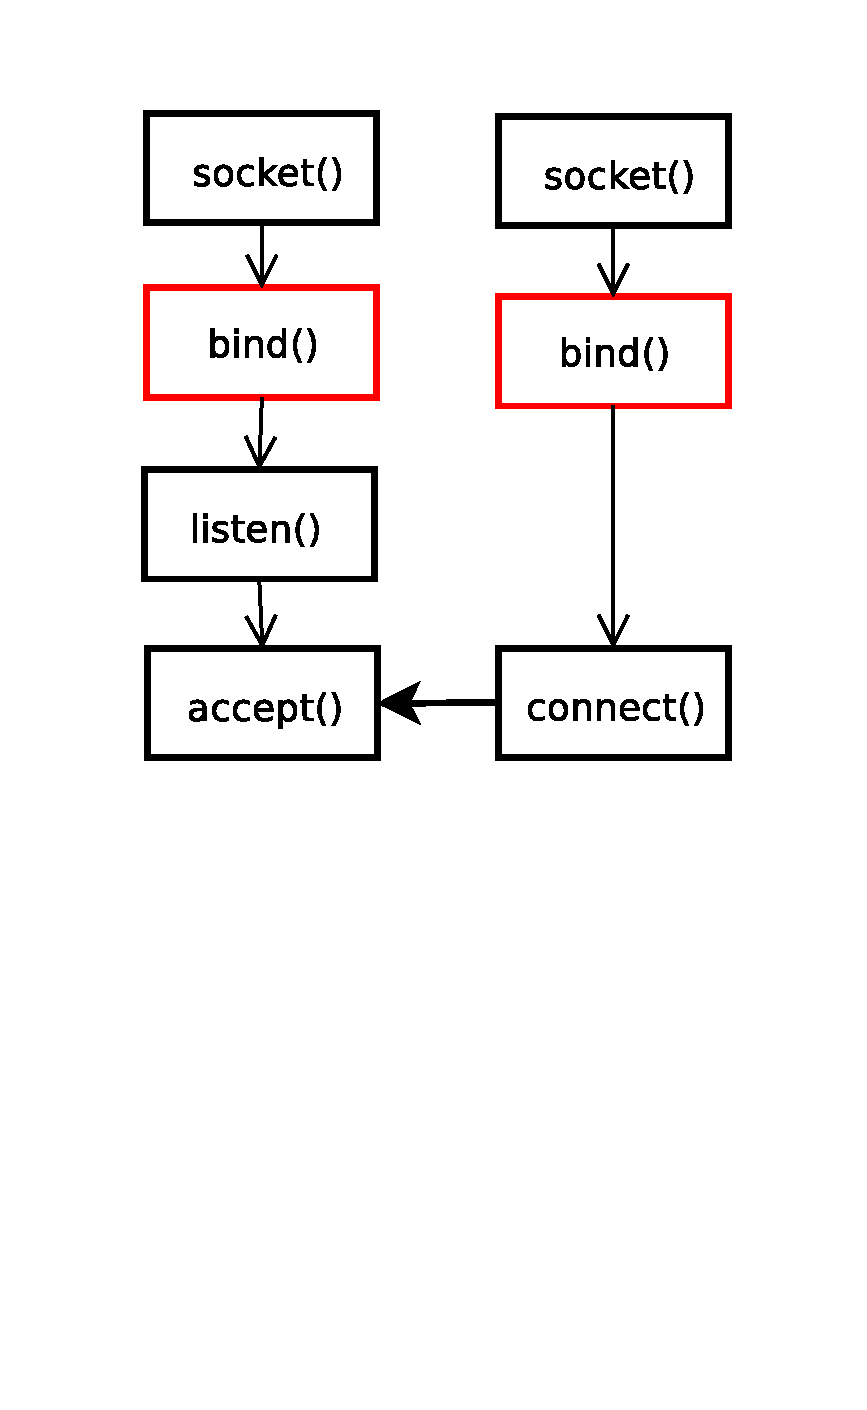
\includegraphics[scale=0.30]{figures/sockets4.eps}
\end{figure}
\end{frame}

\begin{frame}
\frametitle{V4VSockets -- Message Exchange}
%\begin{columns}
%\column{.8\textwidth}
\begin{figure}
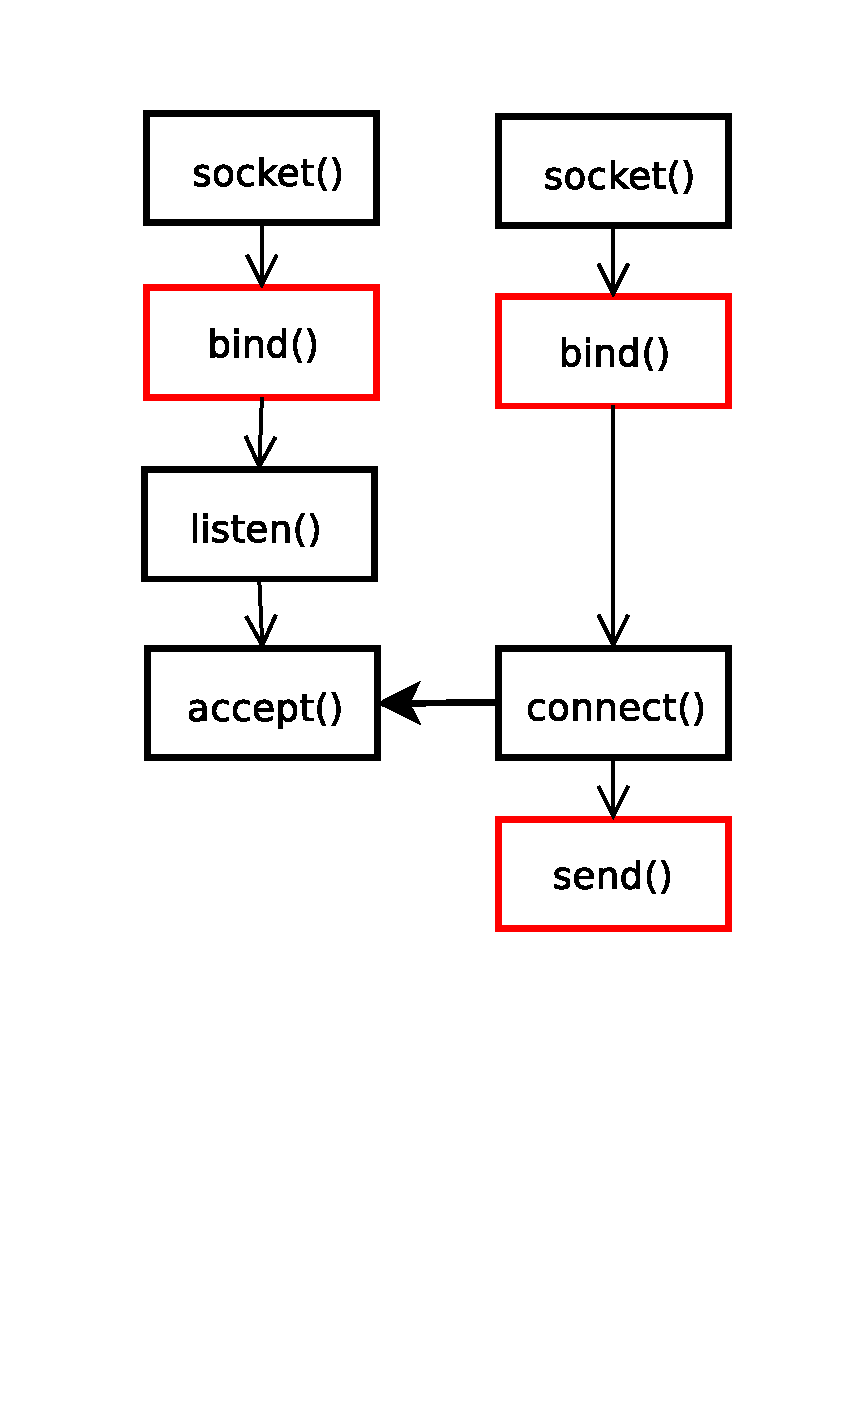
\includegraphics[scale=0.30]{figures/sockets3.eps}
\end{figure}
\end{frame}

\begin{frame}
\frametitle{V4VSockets -- Message Exchange}
\begin{figure}
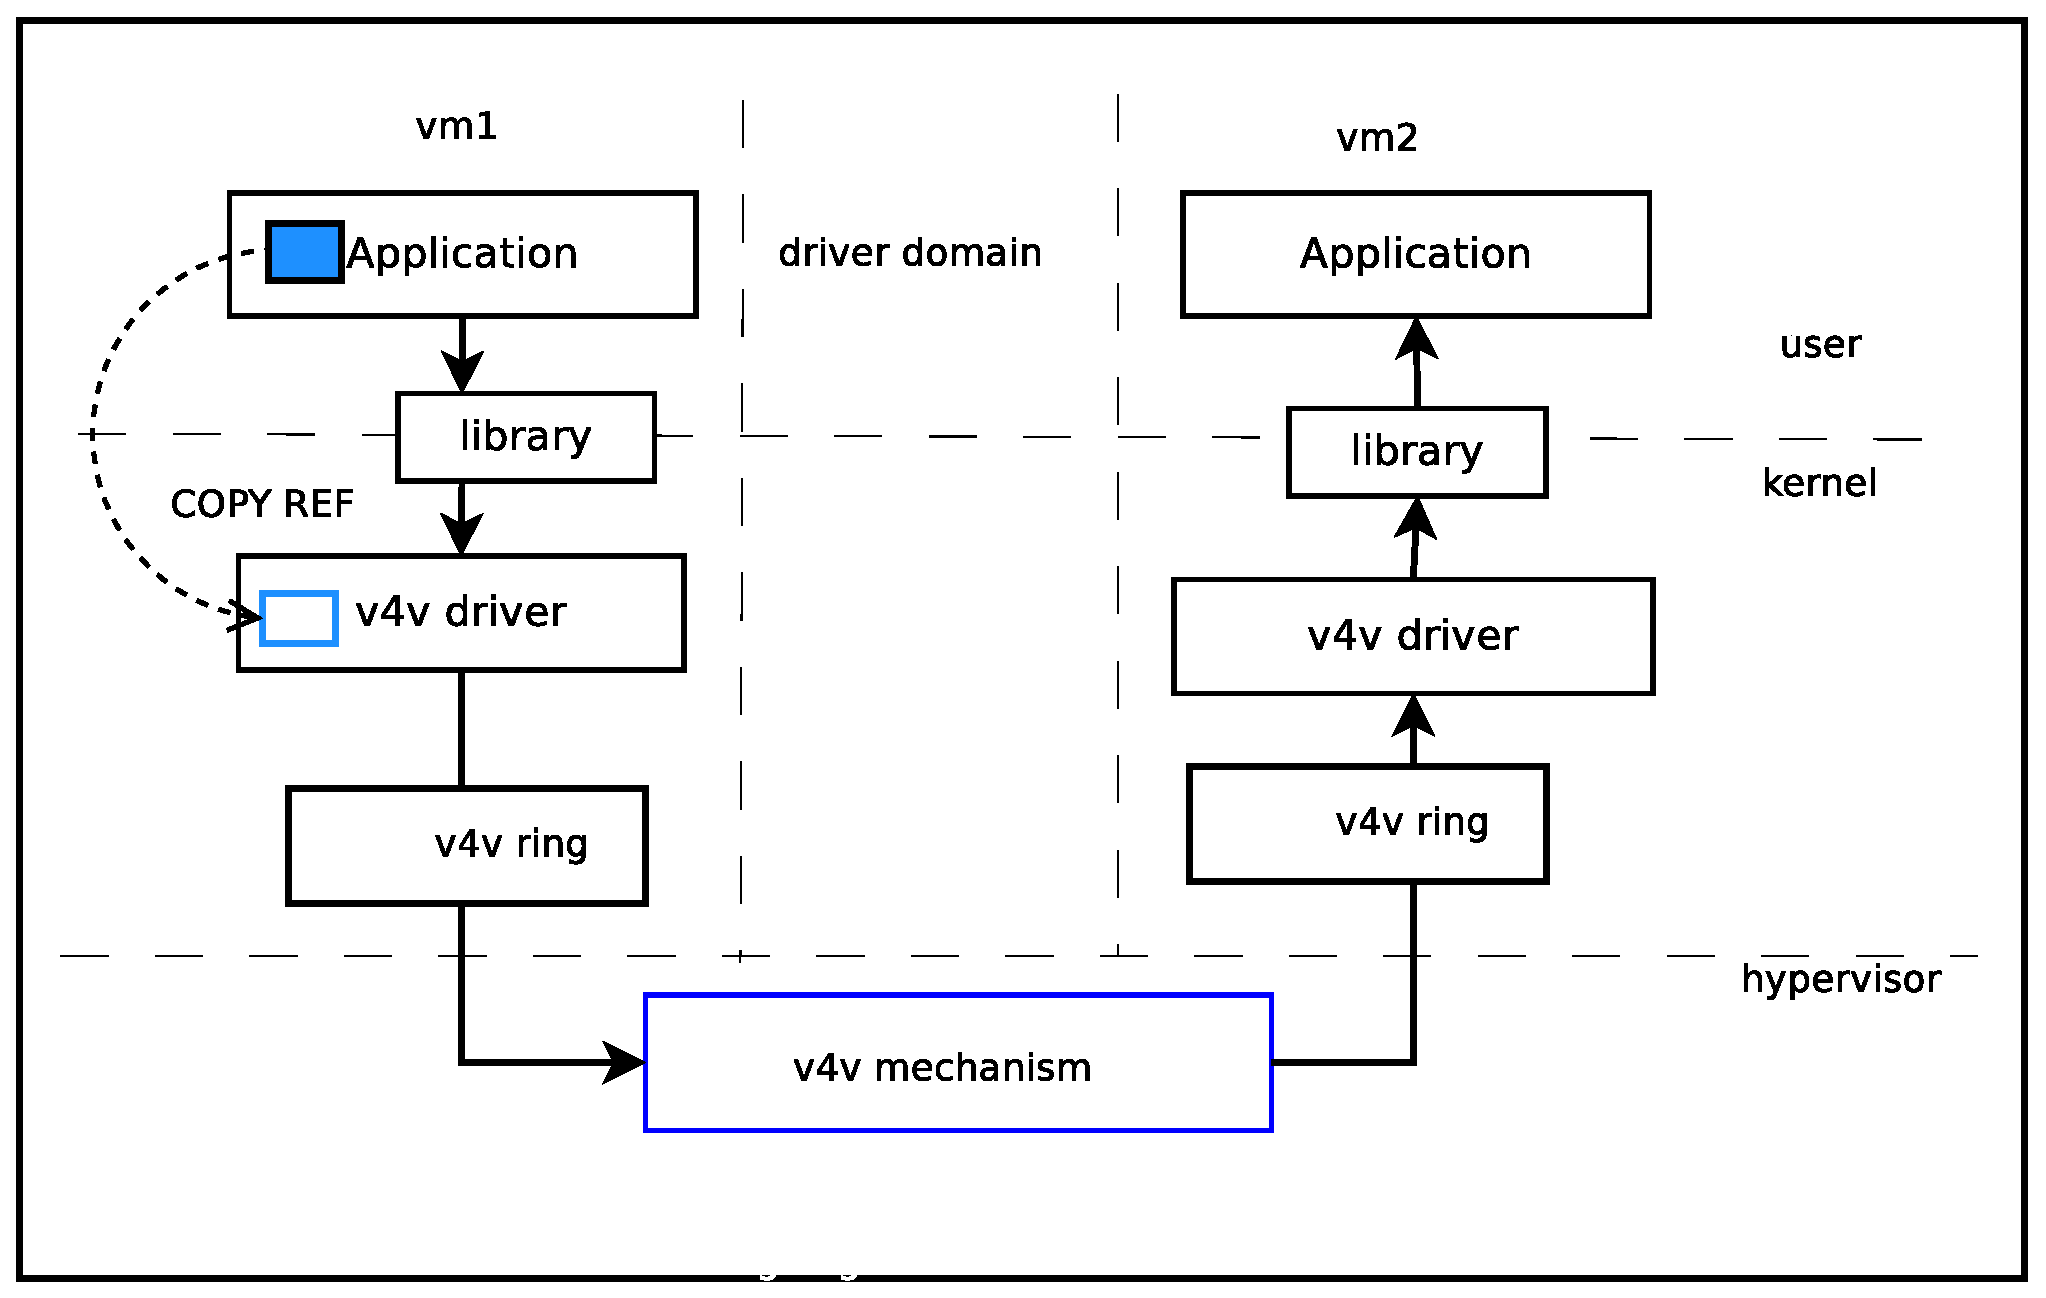
\includegraphics[scale=0.30]{figures/v4vsockets4.eps}
\end{figure}
\end{frame}

\begin{frame}
\frametitle{V4VSockets -- Message Exchange}
\begin{figure}
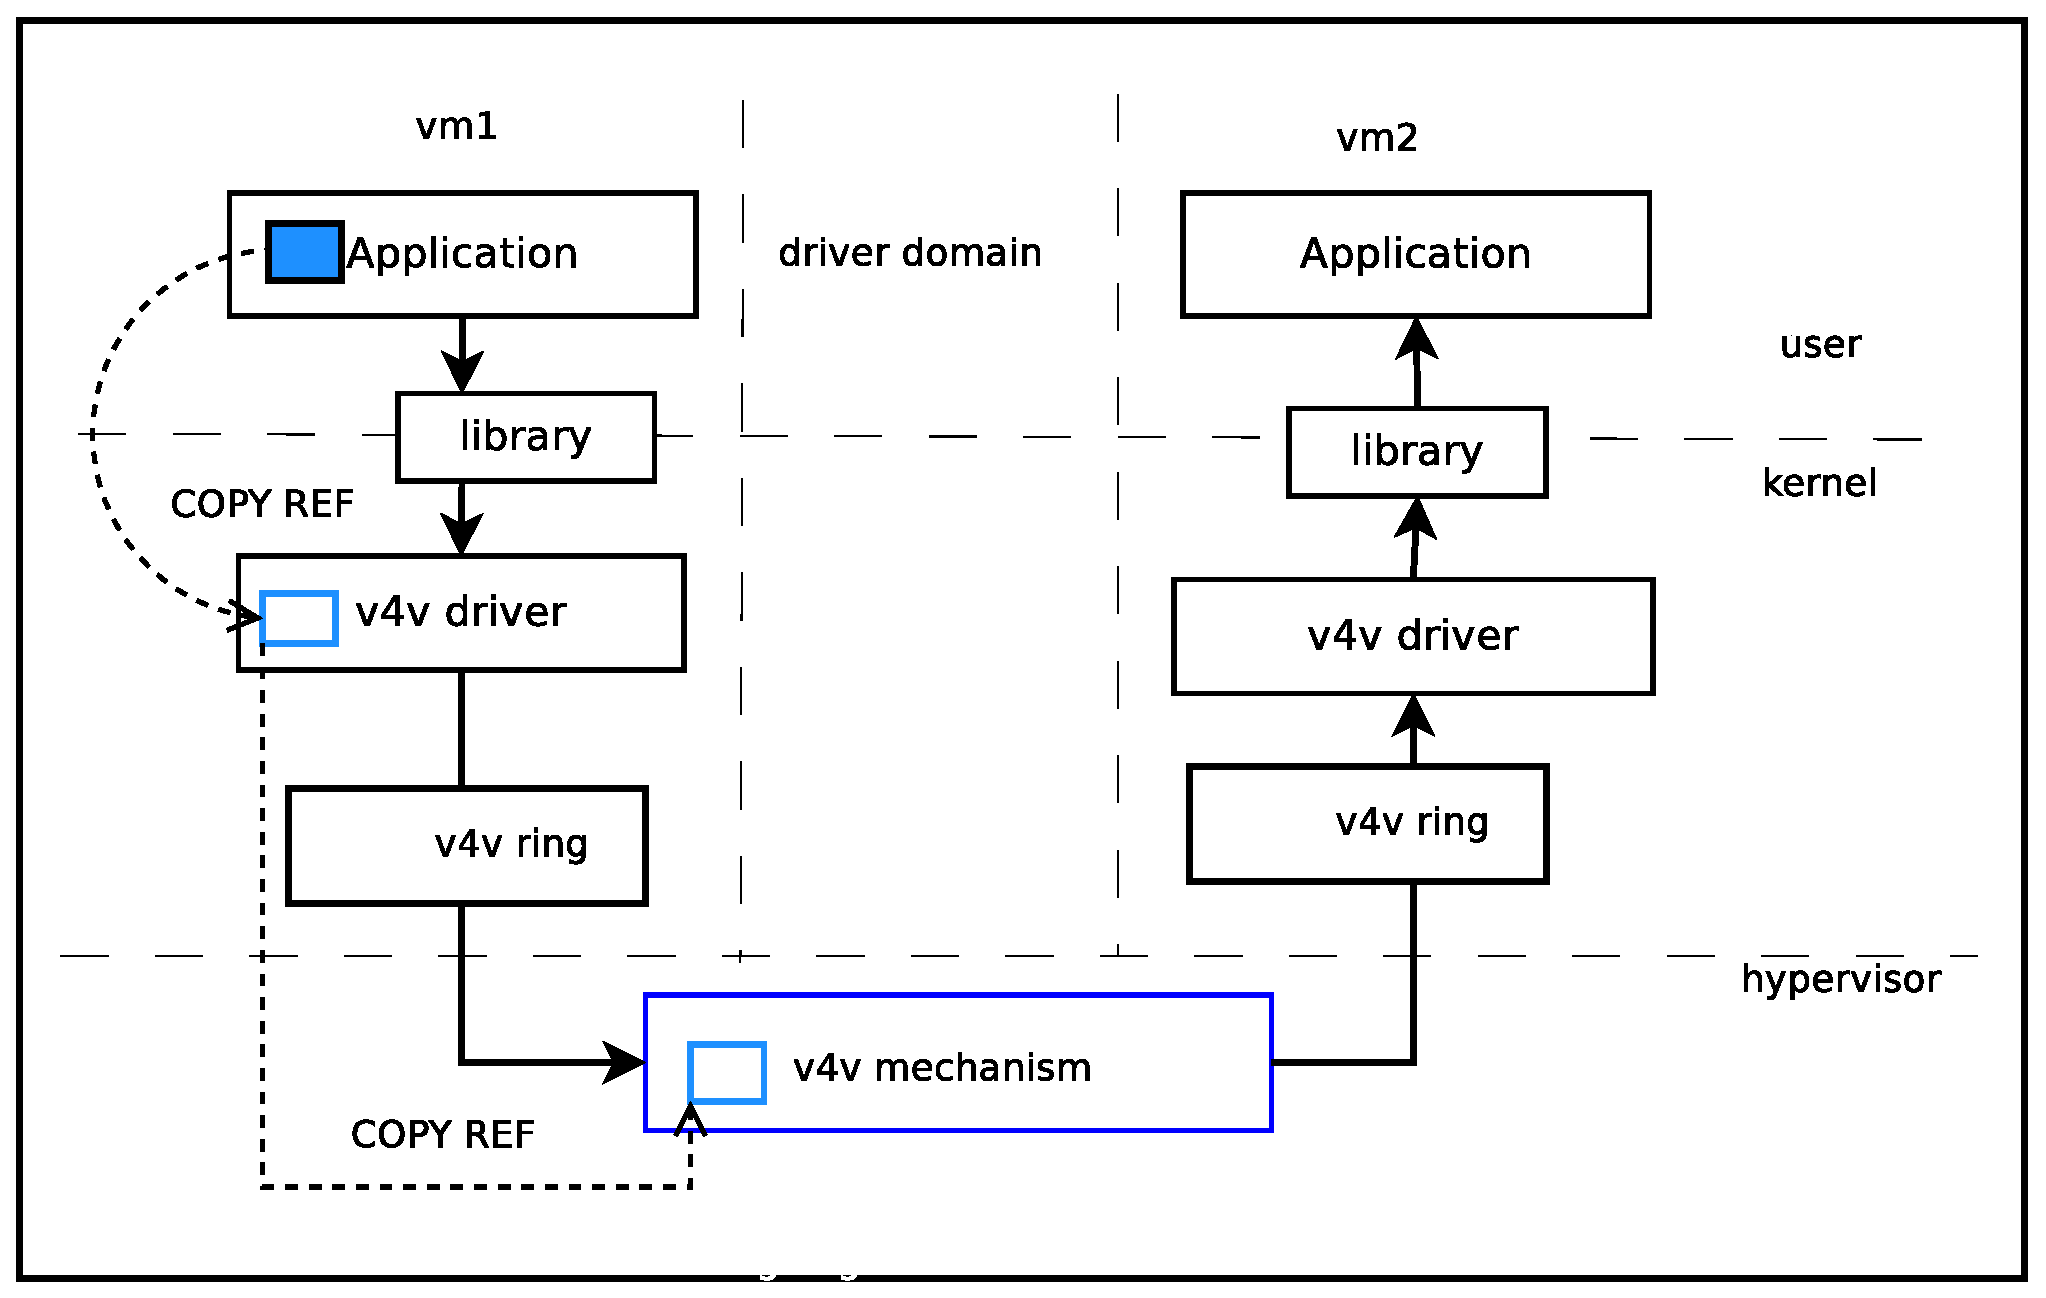
\includegraphics[scale=0.30]{figures/v4vsockets3.eps}
\end{figure}
\end{frame}


\begin{frame}
\frametitle{V4VSockets -- Message Exchange}
%\begin{columns}
%\column{.8\textwidth}
\begin{figure}
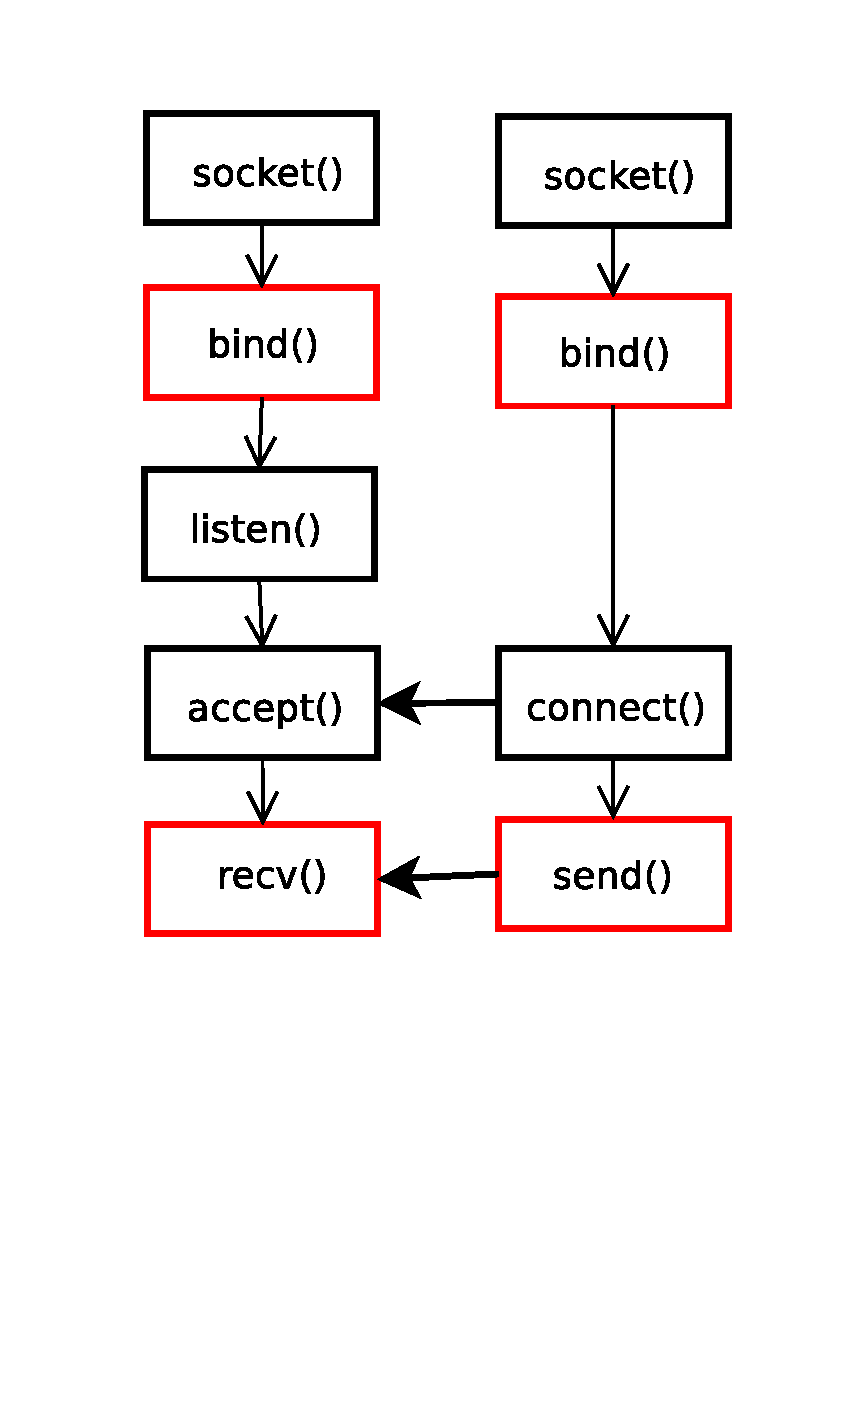
\includegraphics[scale=0.30]{figures/sockets2.eps}
\end{figure}
\end{frame}

\begin{frame}
\frametitle{V4VSockets -- Message Exchange}
\begin{figure}
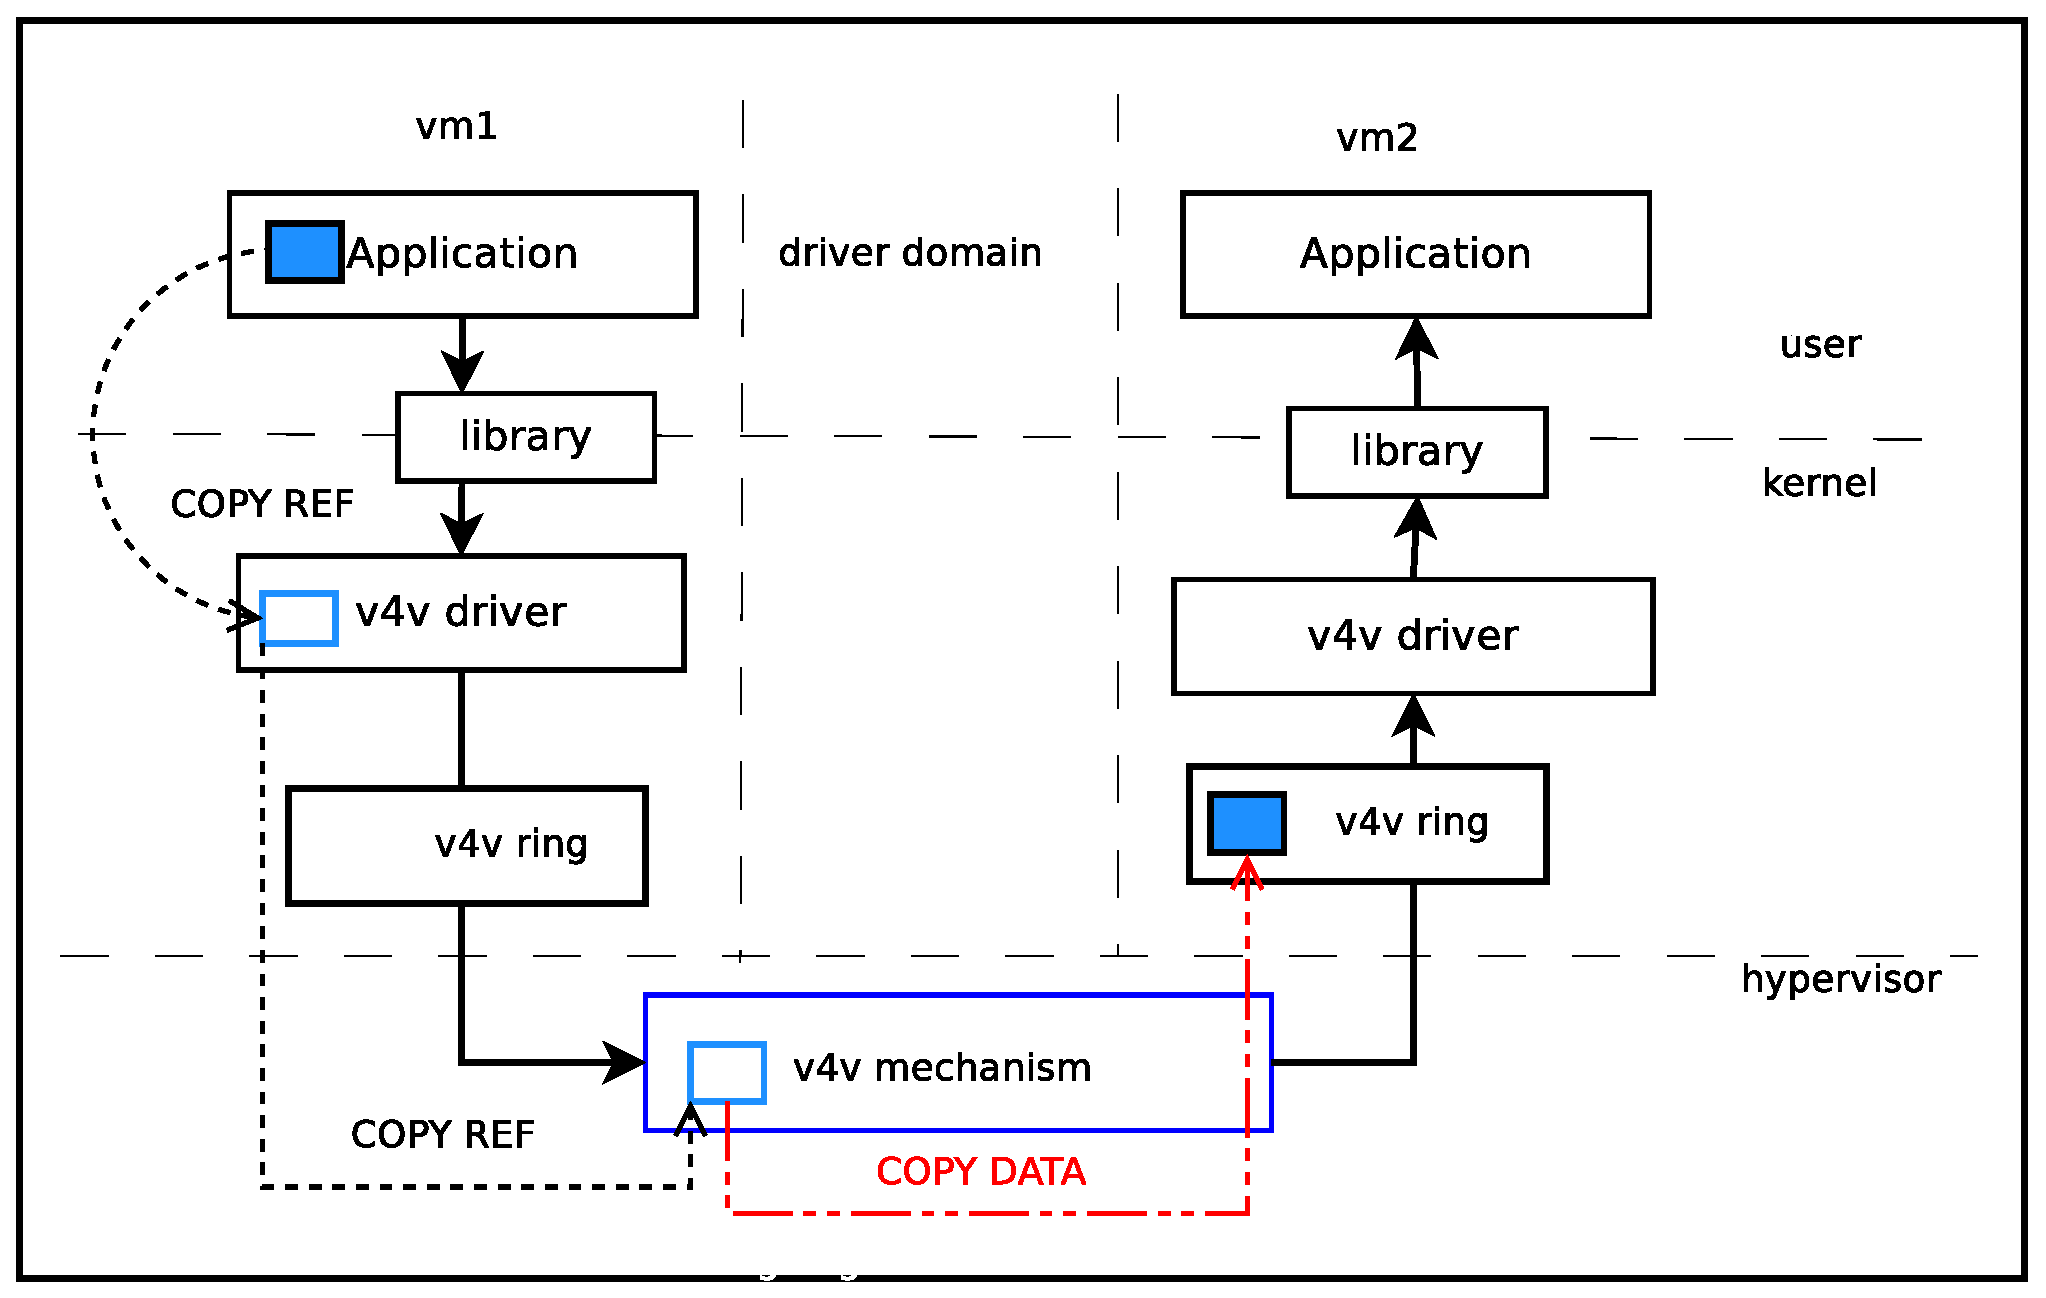
\includegraphics[scale=0.30]{figures/v4vsockets2.eps}
\end{figure}
\end{frame}

\begin{frame}
\frametitle{V4VSockets -- Message Exchange}
\begin{figure}
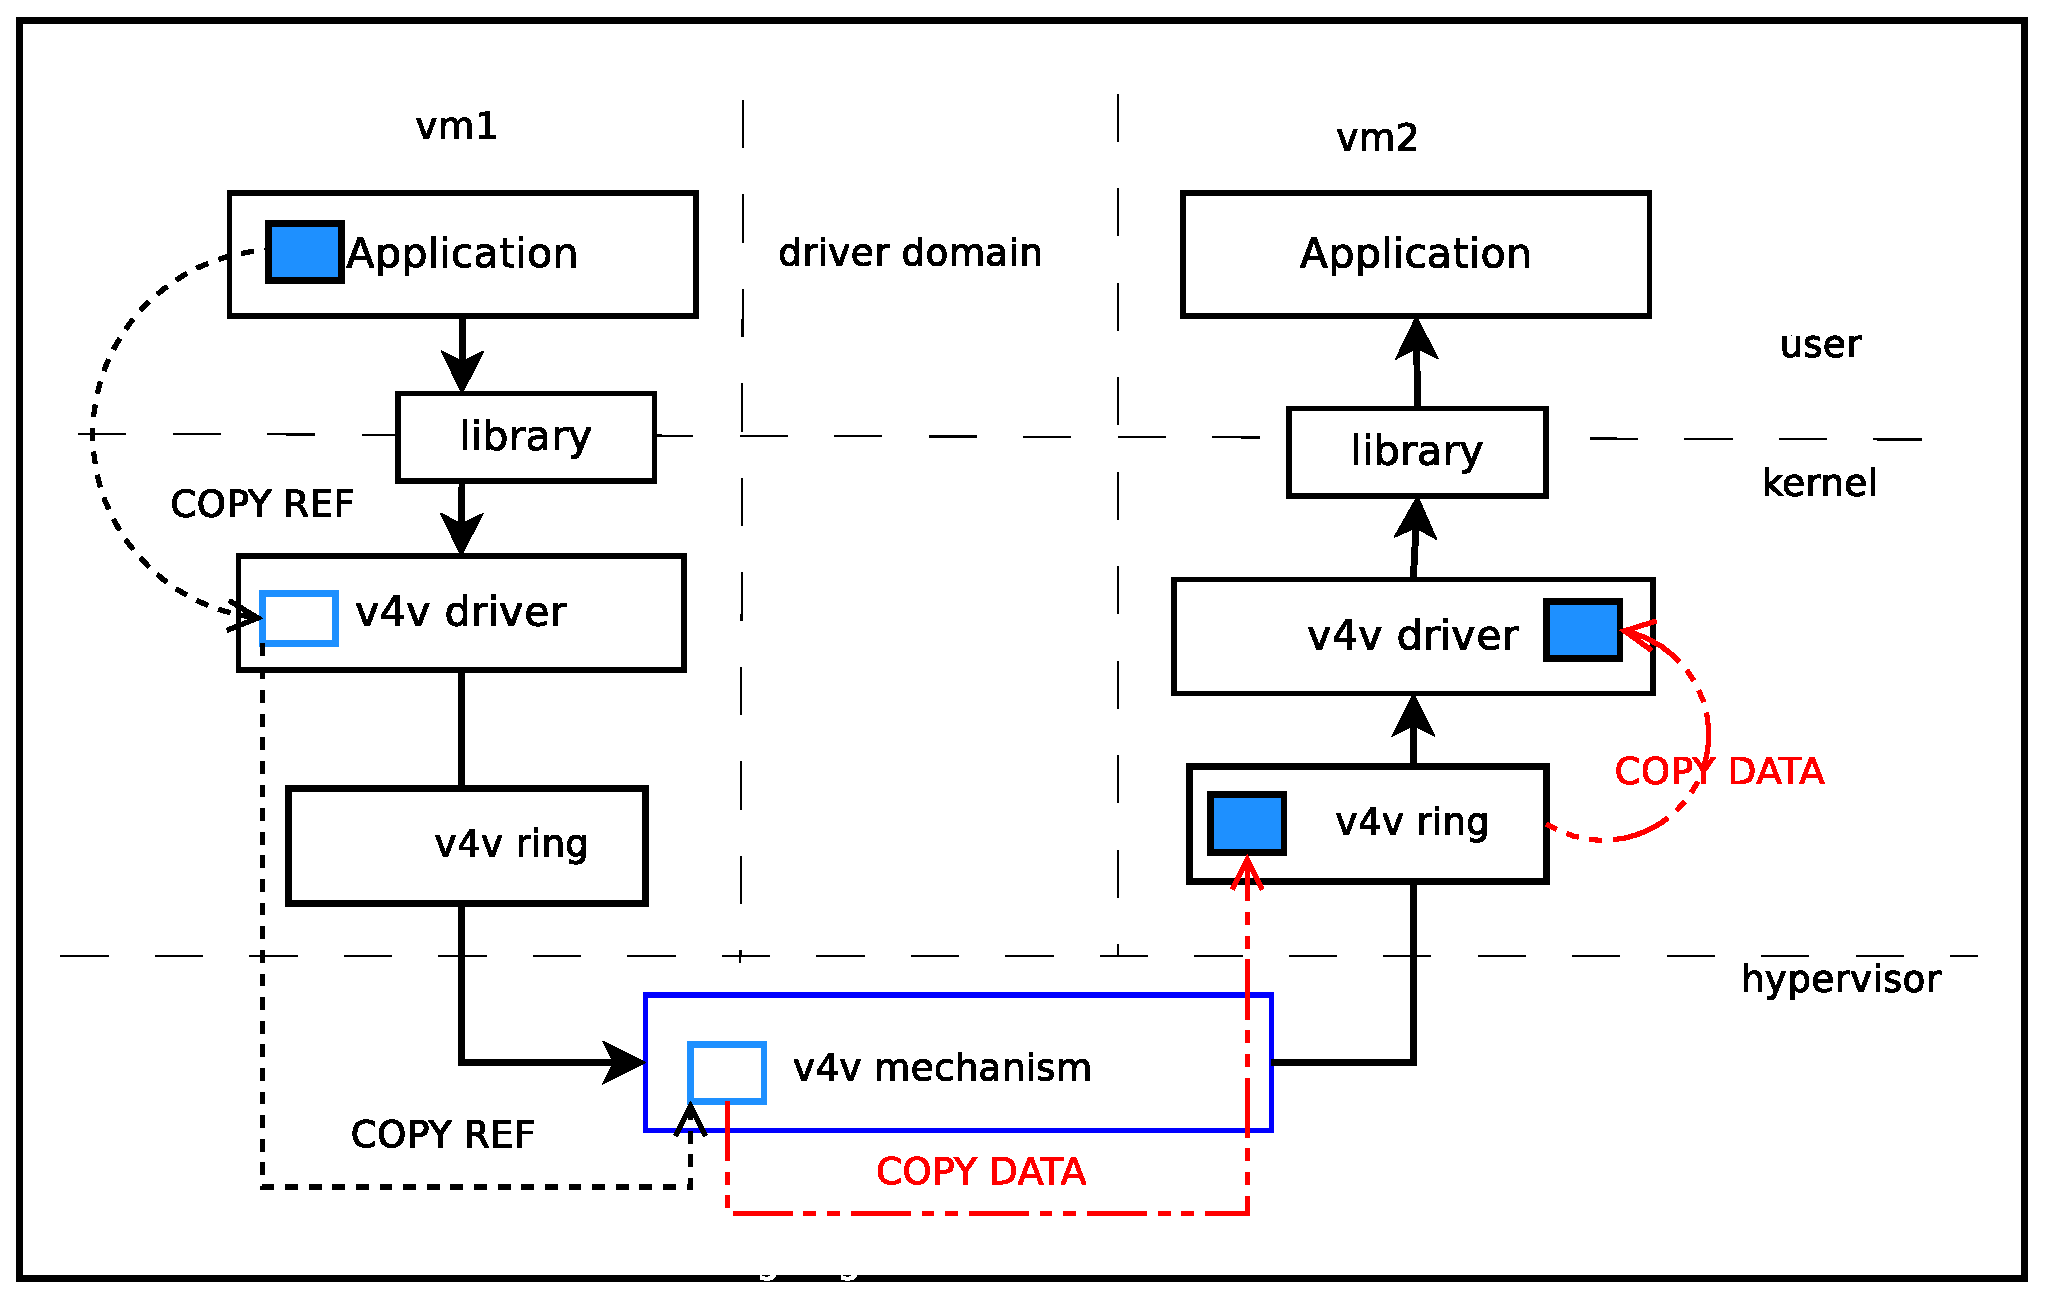
\includegraphics[scale=0.30]{figures/v4vsockets1.eps}
\end{figure}
\end{frame}

\begin{frame}
\frametitle{V4VSockets -- Message Exchange}
\begin{figure}
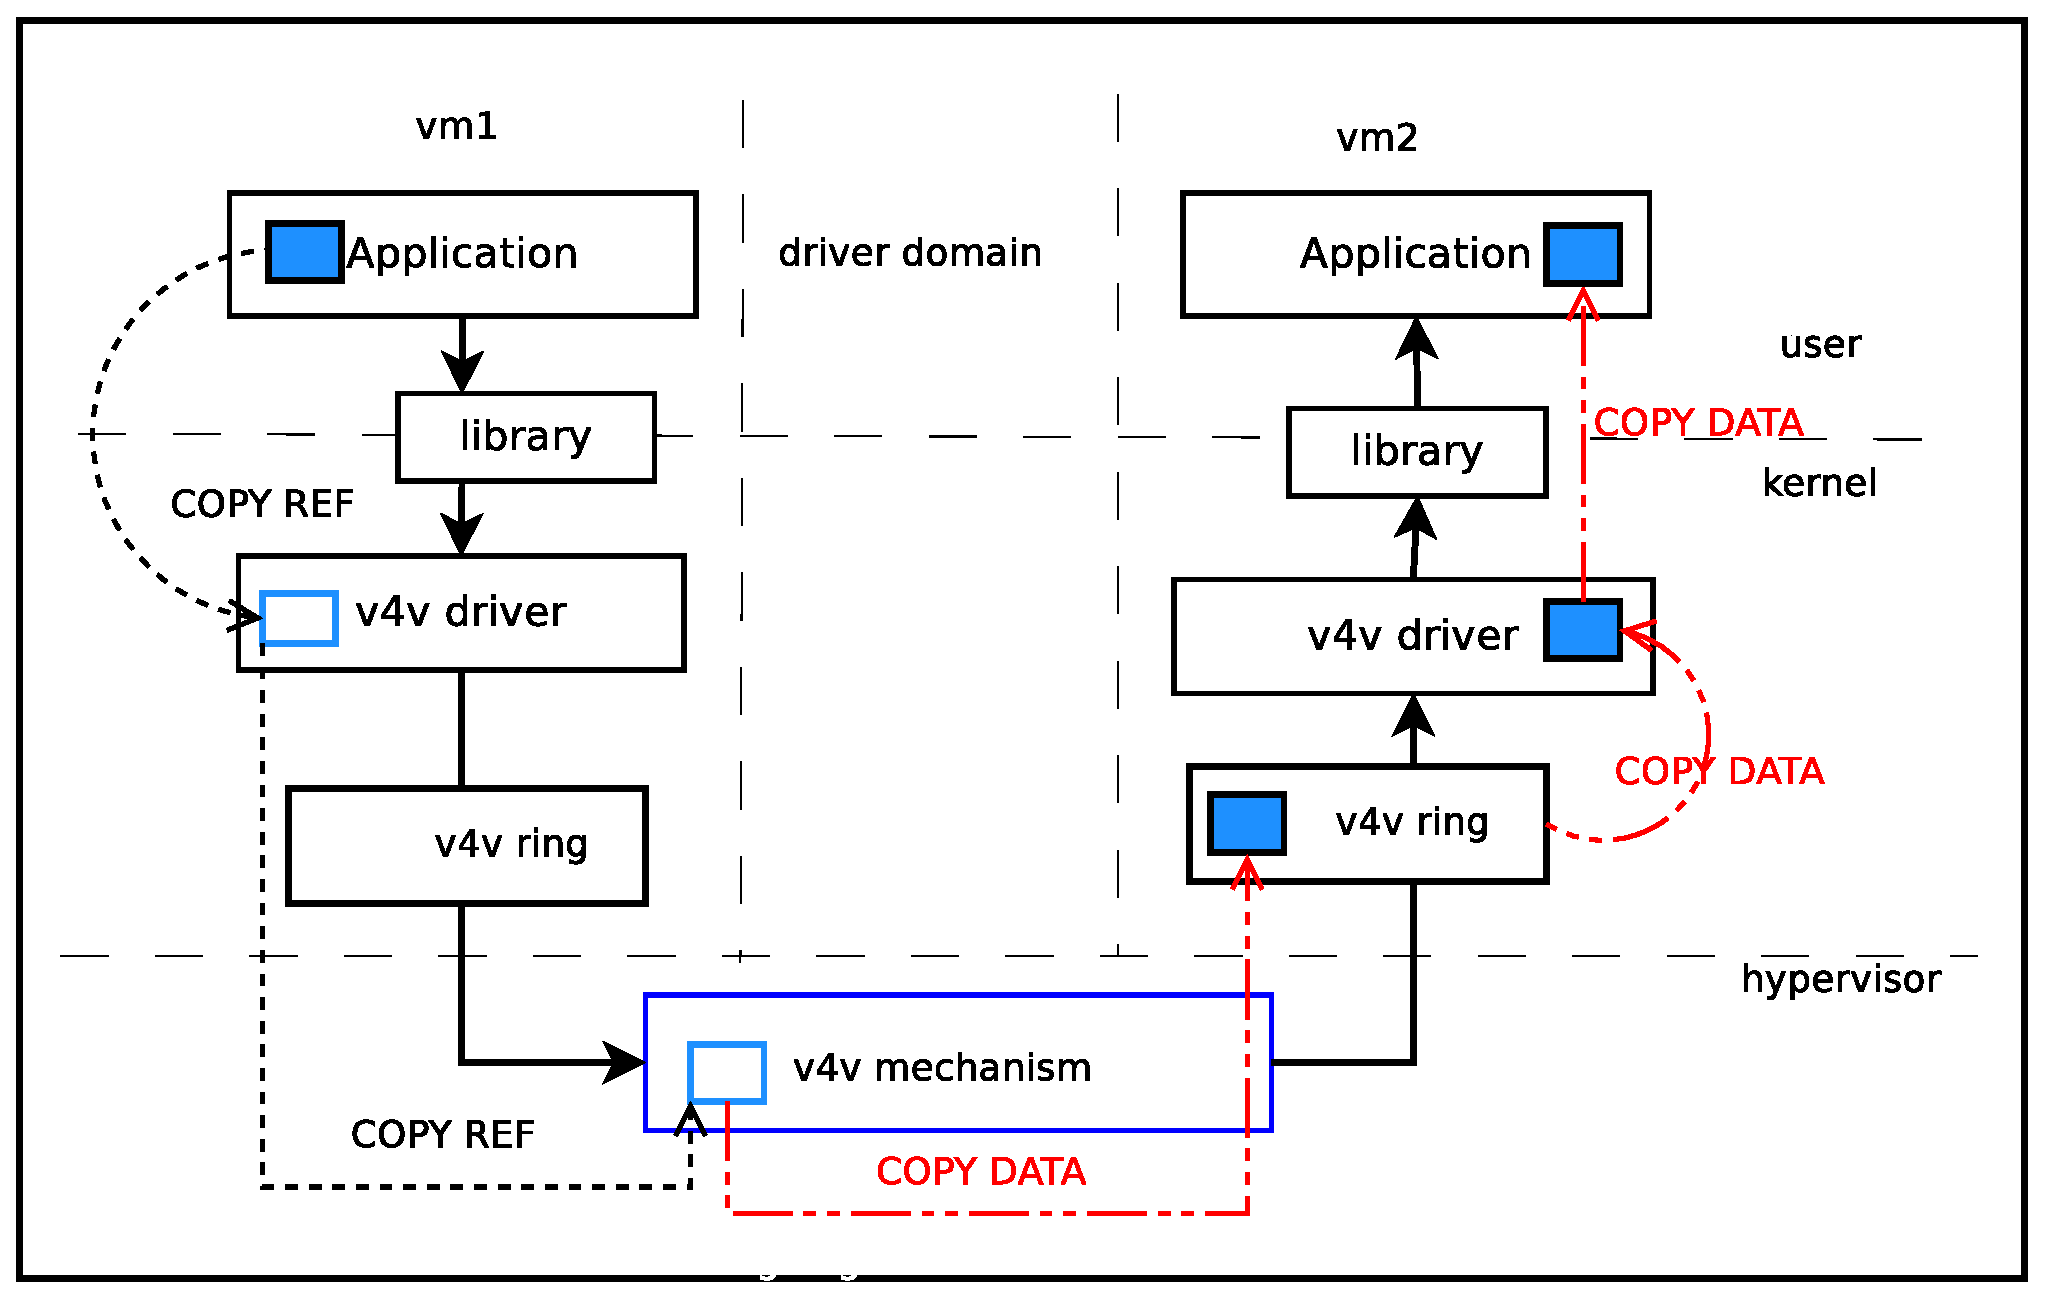
\includegraphics[scale=0.30]{figures/v4vsockets.eps}
\end{figure}
\end{frame}



\begin{frame}
\frametitle{V4VSockets -- Message Exchange}
\begin{figure}
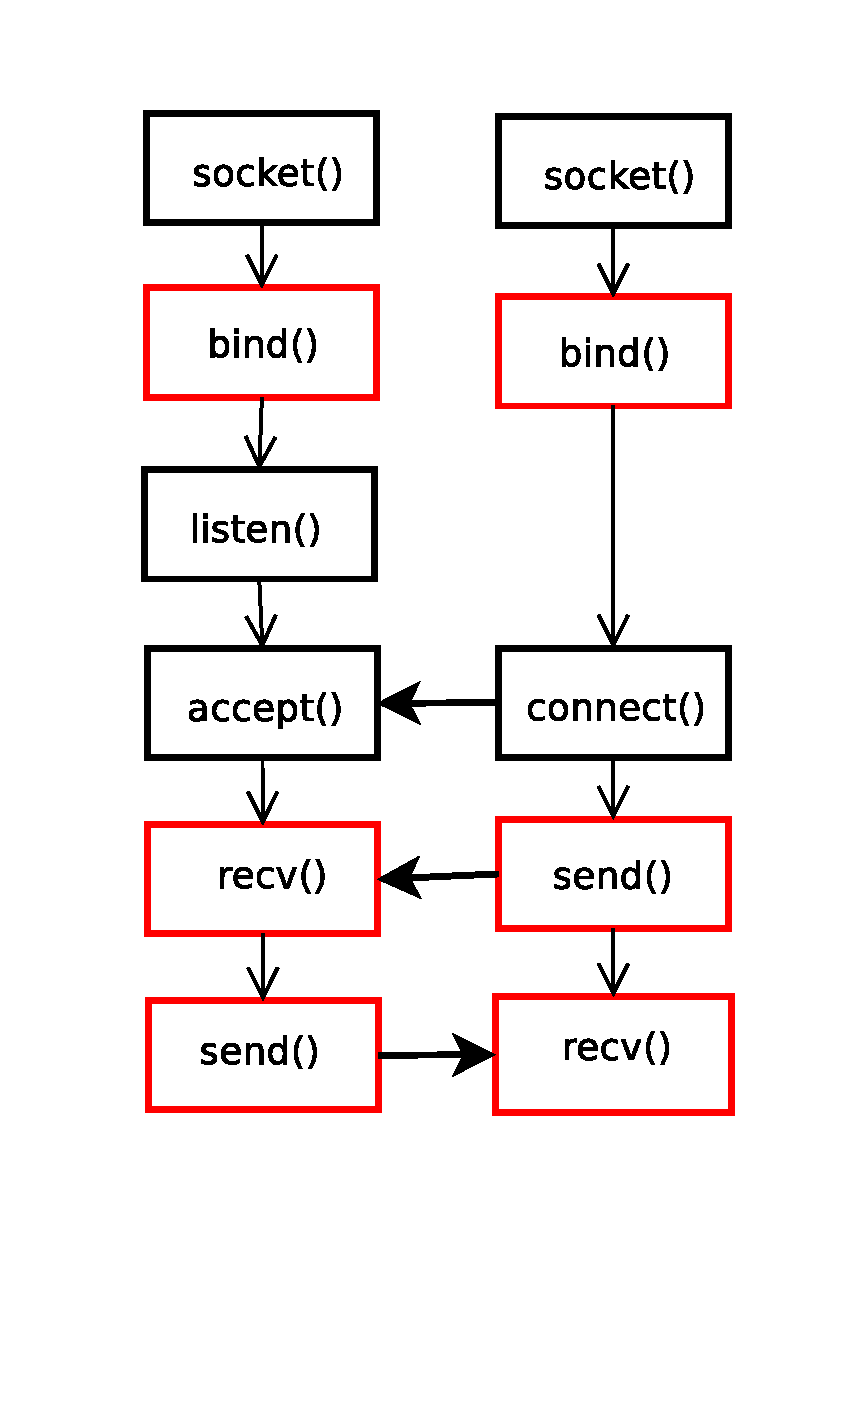
\includegraphics[scale=0.30]{figures/sockets1.eps}
\end{figure}
\end{frame}

\begin{frame}
\frametitle{V4VSockets -- Message Exchange}
\begin{figure}
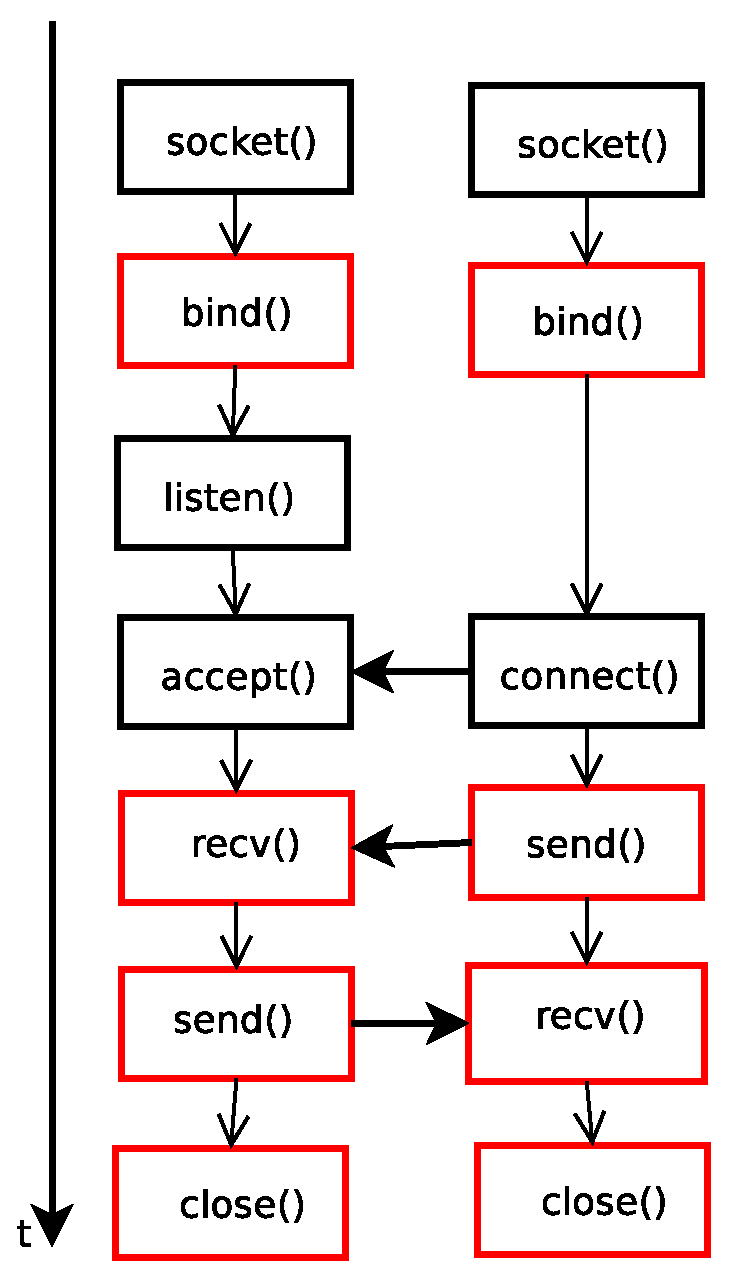
\includegraphics[scale=0.30]{figures/sockets.eps}
\end{figure}
\end{frame}

\subsection{Experimental Evaluation}

\begin{frame}
\frametitle{Performance Results}
\begin{block}{Testbed}
\begin{itemize}
\item 2x \{Intel Xeon @2.4Ghz\}, Intel 5520, 48GB memory, Generic 10GbE
\item Xen 4.5-unstable, Debian GNU/Linux (Linux kernel 3.14.2)
\item generic micro-benchmark: \texttt{pingpong}
%\begin{itemize}
%\item[\tiny{$\leq$ 64b}]: copying
%\item[\tiny{$\leq$ 32KB}]: send \& receive queues
%\item[\tiny{$\geq$ 64KB}]: rendez-vous semantics
%\item$\leq$ 64b: αντιγραφή
%\item$\leq$ 32KB: ουρές αποστολής \& λήψης
%\item$\geq$ 64KB: σημασιολογία rendez-vous
%\end{itemize}
\end{itemize}
\end{block}
%\begin{block}
{Cases:}
\begin{itemize}
\item TCP/UDP sockets
\item V4V Stream/Datagram 
\end{itemize}
%\end{block}
\end{frame}


\begin{frame}
\frametitle{Experimental evaluation -- RTT latency}
\begin{columns}
\column{.8\textwidth}
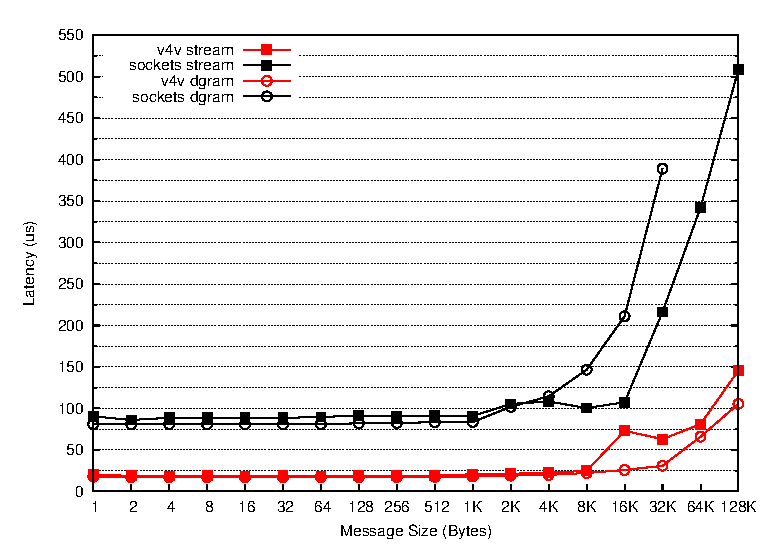
\includegraphics[width=\textwidth]{figures/latencya.eps}
\end{columns}
\end{frame}

\begin{frame}
\frametitle{Experimental evaluation -- Bandwidth}
\begin{columns}
\column{.8\textwidth}
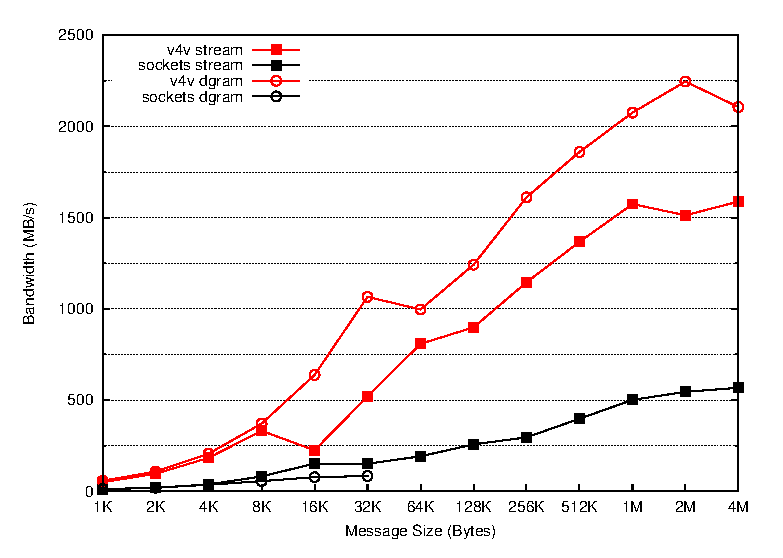
\includegraphics[width=\textwidth]{figures/asdf.eps}
\end{columns}
\end{frame}

%\begin{frame}
%\frametitle{Πειραματική αποτίμηση -- μηνύματα 512K}
%\begin{columns}
%\column{.8\textwidth}
%\includegraphics[width=\textwidth]{figs/bare/aggregate_doms_cpu.eps}
%\end{columns}
%\end{frame}

\begin{frame}
\frametitle{Experimental evaluation -- Scaling factor (up to 16 VMs)}
\begin{columns}
\column{.8\textwidth}
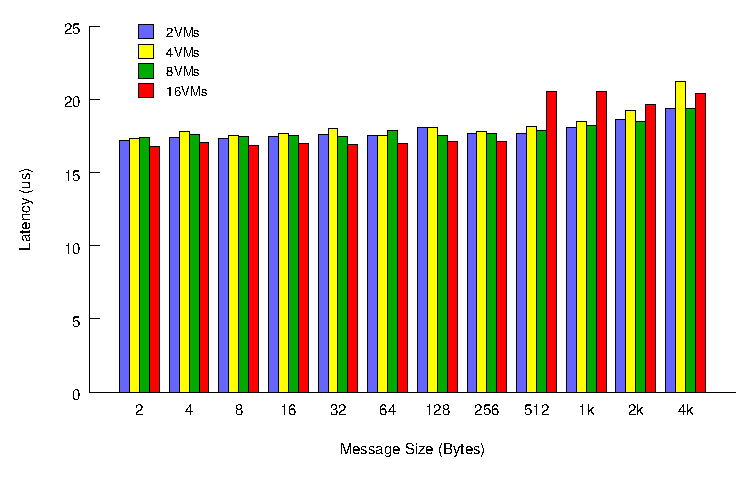
\includegraphics[width=\textwidth]{figures/lat_stream_scale.eps}
\end{columns}

\end{frame}
\begin{frame}
\frametitle{Experimental evaluation -- Scaling factor (up to 16 VMs)}
\begin{columns}
\column{.8\textwidth}
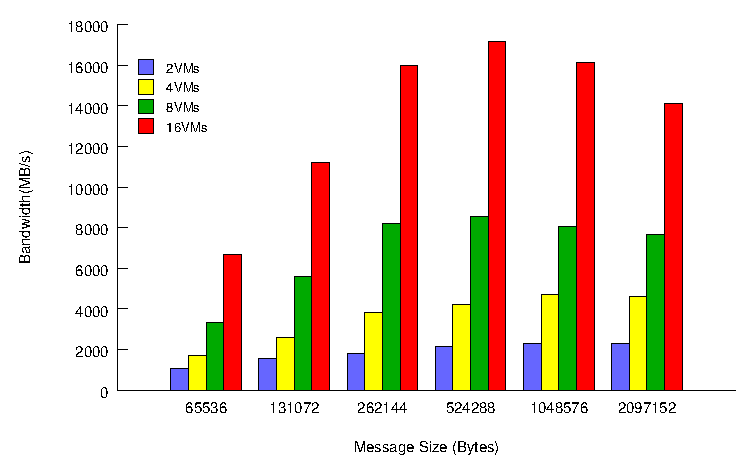
\includegraphics[width=\textwidth]{figures/bw_stream_scale.eps}
\end{columns}
\end{frame}

\section*{Conclusions}

\subsection*{Summary}

\begin{frame}
\frametitle{Summary}
\begin{block}{Intra-node communication in VM environments}
\begin{itemize}
\item split driver model -- generic
\item V4VSockets: framework for low-overhead intra-node communication
\begin{itemize}
\item is not based on a driver domain
\item does not use shared memory between guests (map/grant mechanism)
\item uses memory copies, hypercalls and event channels
%πρωτόκολλο διασύνδεσης σχεδιασμένο για εικονικά περιβάλλοντα
\end{itemize}
\end{itemize}
\end{block}
%\begin{block}{V4VSockets}
\begin{itemize}
\item better throughput (efficient data path, bypass the complex TCP/IP stack)
\item hypercall overheads (small, negligible if correctly finetuned)
\item scalability (no privileged guest involved in communication)
\item isolation (no shared memory)
\item extensible %(layered design, χωρισμένο σε link layer και protocol layer).
%\item hypervisor-specific transport layer, generic interface
%πρωτόκολλο διασύνδεσης σχεδιασμένο για εικονικά περιβάλλοντα
\end{itemize}
%\end{block}
\end{frame}

\begin{frame}
\frametitle{Future endaevors}
\begin{itemize}
%\item ένταξη σημασιολογίας δικτύων υψηλής επίδοσης στο μοντέλο διαχωρισμένου οδηγού
%\item επικοινωνία με πολύ χαμηλό χρόνο απόκρισης και υψηλή ρυθμαπόδοση -- συγκρίσιμα με περιβάλλοντα χωρίς virtualization
%\item συμβατότητα με πρωτόκολλα ανώτερων στρωμάτων (MPI κλπ.)
\item cpu utilization overheads
\item NUMA and multihierarchical memory architectures
\item map instead of copy (study the systems behavior of providing a shared memory space between VMs)
\item Optimize away copies on the data path.
\end{itemize}
%\begin{block}{Future Plans:}
%\begin{itemize}
%\item optimize Xen2MX to reach native performance numbers
%\item generalize the case to different hypervisors
%\end{itemize}
%\end{block}

Available online as open-source \url{https://github.com/HPSI/V4VSockets}

\end{frame}
%
\begin{frame}
\frametitle{Thanks!}
                \vfill%
\begin{columns}
        \column{.35\textwidth}
        \begin{center}
                %\vfill%
            %    \begin{block}{}
        \begin{center}
                        {\LARGE Questions?}
        \end{center}
             %   \end{block}
                \vfill%
                %\vfill%
        \end{center}
\end{columns}
                \vfill%
\end{frame}


\begin{frame}
\frametitle{}
                \vfill%
\begin{columns}
        \column{.35\textwidth}
        \begin{center}
                %\vfill%
            %    \begin{block}{}
             %   \end{block}
                \vfill%
                %\vfill%
        \end{center}
\end{columns}
                \vfill%
\end{frame}
%
\begin{frame}
\frametitle{}
                \vfill%
\begin{columns}
        \column{.35\textwidth}
        \begin{center}
                %\vfill%
            %    \begin{block}{}
        \begin{center}
                        {\LARGE Backup}
        \end{center}
             %   \end{block}
                \vfill%
                %\vfill%
        \end{center}
\end{columns}
                \vfill%
\end{frame}

\begin{frame}
\frametitle{Experimental evaluation -- 2M message size vs Hypercalls}
\begin{columns}
\column{.8\textwidth}
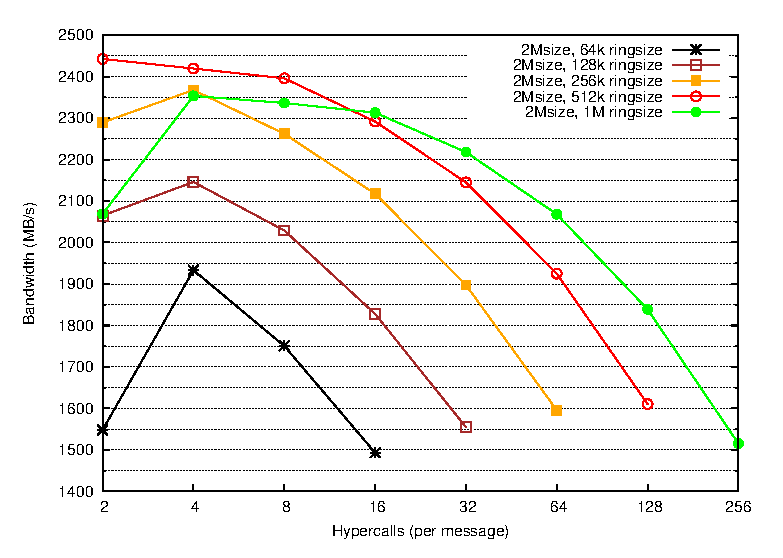
\includegraphics[width=\textwidth]{figures/2M.eps}
\end{columns}
\end{frame}

\begin{frame}
\frametitle{Experimental evaluation -- Datagram scalability}
\begin{columns}
\column{.8\textwidth}
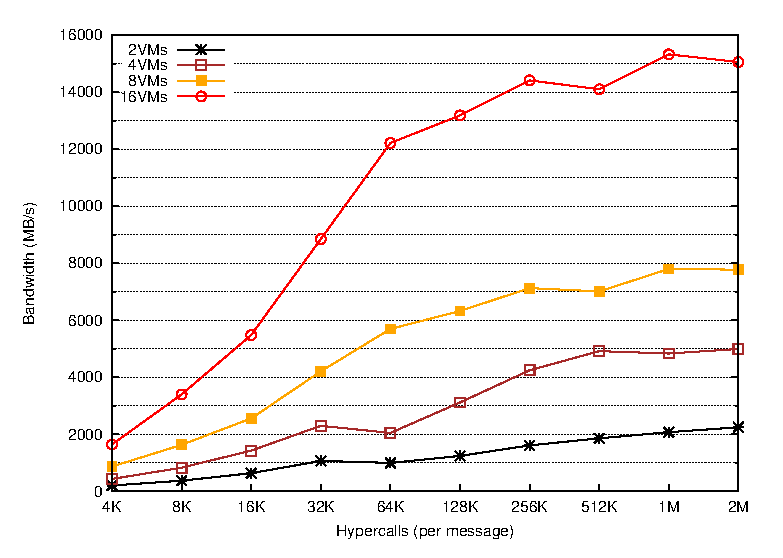
\includegraphics[width=\textwidth]{figures/bw_dgram_scale.eps}
\end{columns}
\end{frame}

\begin{frame}
\frametitle{Experimental evaluation -- Hypercalls per message}
\begin{columns}
\column{.8\textwidth}
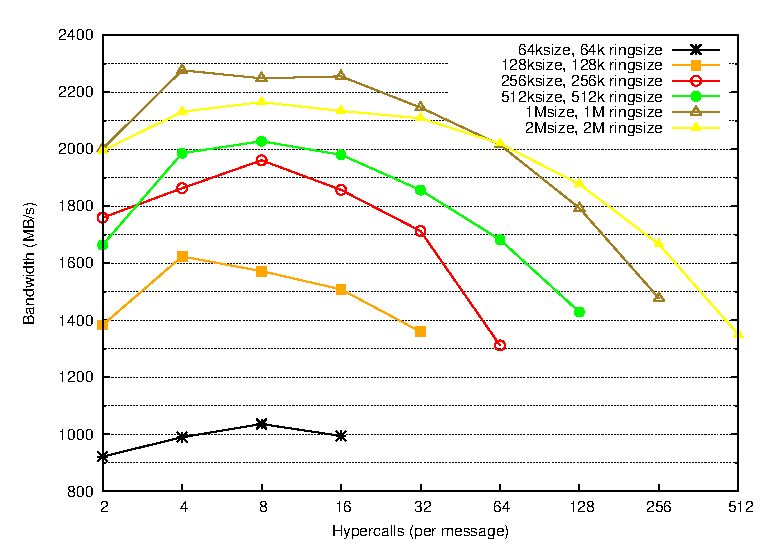
\includegraphics[width=\textwidth]{figures/mix.eps}
\end{columns}
\end{frame}
%
%\begin{frame}
%\frametitle{Πειραματική αποτίμηση -- Ποσοστό χρήσης CPU για το VM}
%\begin{columns}
%\column{.8\textwidth}
%\includegraphics[width=\textwidth]{figs/bare/lat_breakdown_domU.eps}
%\end{columns}
%\end{frame}
%
%\begin{frame}
%\frametitle{Xen2MX -- I}
%\begin{columns}
%\column{.8\textwidth}
%\includegraphics[width=\textwidth]{figs/bare/xen2mx_step1.pdf}
%\end{columns}
%\end{frame}
%
%\begin{frame}
%\frametitle{Xen2MX -- II}
%\begin{columns}
%\column{.8\textwidth}
%\includegraphics[width=\textwidth]{figs/bare/xen2mx_step2.pdf}
%\end{columns}
%\end{frame}
%
%\begin{frame}
%\frametitle{Xen2MX -- III}
%\begin{columns}
%\column{.8\textwidth}
%\includegraphics[width=\textwidth]{figs/bare/xen2mx_step3.pdf}
%\end{columns}
%\end{frame}
%
%\begin{frame}
%\frametitle{Xen2MX -- IV (Bridged)}
%\begin{columns}
%\column{.8\textwidth}
%\includegraphics[width=\textwidth]{figs/bare/xen2mx_step4.pdf}
%\end{columns}
%\end{frame}
%
%\begin{frame}
%\frametitle{Xen2MX -- ΙV (IOV)}
%\begin{columns}
%\column{.8\textwidth}
%\includegraphics[width=\textwidth]{figs/bare/xen2mx_step5.pdf}
%\end{columns}
%\end{frame}
%
%\begin{frame}
%\frametitle{Xen2MX -- IV (Xen2MX)}
%\begin{columns}
%\column{.8\textwidth}
%\includegraphics[width=\textwidth]{figs/bare/xen2mx_step6.pdf}
%\end{columns}
%\end{frame}
%
\end{document}
